% Options for packages loaded elsewhere
\PassOptionsToPackage{unicode}{hyperref}
\PassOptionsToPackage{hyphens}{url}
%
\documentclass[
]{book}
\usepackage{amsmath,amssymb}
\usepackage{lmodern}
\usepackage{iftex}
\ifPDFTeX
  \usepackage[T1]{fontenc}
  \usepackage[utf8]{inputenc}
  \usepackage{textcomp} % provide euro and other symbols
\else % if luatex or xetex
  \usepackage{unicode-math}
  \defaultfontfeatures{Scale=MatchLowercase}
  \defaultfontfeatures[\rmfamily]{Ligatures=TeX,Scale=1}
\fi
% Use upquote if available, for straight quotes in verbatim environments
\IfFileExists{upquote.sty}{\usepackage{upquote}}{}
\IfFileExists{microtype.sty}{% use microtype if available
  \usepackage[]{microtype}
  \UseMicrotypeSet[protrusion]{basicmath} % disable protrusion for tt fonts
}{}
\makeatletter
\@ifundefined{KOMAClassName}{% if non-KOMA class
  \IfFileExists{parskip.sty}{%
    \usepackage{parskip}
  }{% else
    \setlength{\parindent}{0pt}
    \setlength{\parskip}{6pt plus 2pt minus 1pt}}
}{% if KOMA class
  \KOMAoptions{parskip=half}}
\makeatother
\usepackage{xcolor}
\usepackage{color}
\usepackage{fancyvrb}
\newcommand{\VerbBar}{|}
\newcommand{\VERB}{\Verb[commandchars=\\\{\}]}
\DefineVerbatimEnvironment{Highlighting}{Verbatim}{commandchars=\\\{\}}
% Add ',fontsize=\small' for more characters per line
\usepackage{framed}
\definecolor{shadecolor}{RGB}{248,248,248}
\newenvironment{Shaded}{\begin{snugshade}}{\end{snugshade}}
\newcommand{\AlertTok}[1]{\textcolor[rgb]{0.94,0.16,0.16}{#1}}
\newcommand{\AnnotationTok}[1]{\textcolor[rgb]{0.56,0.35,0.01}{\textbf{\textit{#1}}}}
\newcommand{\AttributeTok}[1]{\textcolor[rgb]{0.77,0.63,0.00}{#1}}
\newcommand{\BaseNTok}[1]{\textcolor[rgb]{0.00,0.00,0.81}{#1}}
\newcommand{\BuiltInTok}[1]{#1}
\newcommand{\CharTok}[1]{\textcolor[rgb]{0.31,0.60,0.02}{#1}}
\newcommand{\CommentTok}[1]{\textcolor[rgb]{0.56,0.35,0.01}{\textit{#1}}}
\newcommand{\CommentVarTok}[1]{\textcolor[rgb]{0.56,0.35,0.01}{\textbf{\textit{#1}}}}
\newcommand{\ConstantTok}[1]{\textcolor[rgb]{0.00,0.00,0.00}{#1}}
\newcommand{\ControlFlowTok}[1]{\textcolor[rgb]{0.13,0.29,0.53}{\textbf{#1}}}
\newcommand{\DataTypeTok}[1]{\textcolor[rgb]{0.13,0.29,0.53}{#1}}
\newcommand{\DecValTok}[1]{\textcolor[rgb]{0.00,0.00,0.81}{#1}}
\newcommand{\DocumentationTok}[1]{\textcolor[rgb]{0.56,0.35,0.01}{\textbf{\textit{#1}}}}
\newcommand{\ErrorTok}[1]{\textcolor[rgb]{0.64,0.00,0.00}{\textbf{#1}}}
\newcommand{\ExtensionTok}[1]{#1}
\newcommand{\FloatTok}[1]{\textcolor[rgb]{0.00,0.00,0.81}{#1}}
\newcommand{\FunctionTok}[1]{\textcolor[rgb]{0.00,0.00,0.00}{#1}}
\newcommand{\ImportTok}[1]{#1}
\newcommand{\InformationTok}[1]{\textcolor[rgb]{0.56,0.35,0.01}{\textbf{\textit{#1}}}}
\newcommand{\KeywordTok}[1]{\textcolor[rgb]{0.13,0.29,0.53}{\textbf{#1}}}
\newcommand{\NormalTok}[1]{#1}
\newcommand{\OperatorTok}[1]{\textcolor[rgb]{0.81,0.36,0.00}{\textbf{#1}}}
\newcommand{\OtherTok}[1]{\textcolor[rgb]{0.56,0.35,0.01}{#1}}
\newcommand{\PreprocessorTok}[1]{\textcolor[rgb]{0.56,0.35,0.01}{\textit{#1}}}
\newcommand{\RegionMarkerTok}[1]{#1}
\newcommand{\SpecialCharTok}[1]{\textcolor[rgb]{0.00,0.00,0.00}{#1}}
\newcommand{\SpecialStringTok}[1]{\textcolor[rgb]{0.31,0.60,0.02}{#1}}
\newcommand{\StringTok}[1]{\textcolor[rgb]{0.31,0.60,0.02}{#1}}
\newcommand{\VariableTok}[1]{\textcolor[rgb]{0.00,0.00,0.00}{#1}}
\newcommand{\VerbatimStringTok}[1]{\textcolor[rgb]{0.31,0.60,0.02}{#1}}
\newcommand{\WarningTok}[1]{\textcolor[rgb]{0.56,0.35,0.01}{\textbf{\textit{#1}}}}
\usepackage{longtable,booktabs,array}
\usepackage{calc} % for calculating minipage widths
% Correct order of tables after \paragraph or \subparagraph
\usepackage{etoolbox}
\makeatletter
\patchcmd\longtable{\par}{\if@noskipsec\mbox{}\fi\par}{}{}
\makeatother
% Allow footnotes in longtable head/foot
\IfFileExists{footnotehyper.sty}{\usepackage{footnotehyper}}{\usepackage{footnote}}
\makesavenoteenv{longtable}
\usepackage{graphicx}
\makeatletter
\def\maxwidth{\ifdim\Gin@nat@width>\linewidth\linewidth\else\Gin@nat@width\fi}
\def\maxheight{\ifdim\Gin@nat@height>\textheight\textheight\else\Gin@nat@height\fi}
\makeatother
% Scale images if necessary, so that they will not overflow the page
% margins by default, and it is still possible to overwrite the defaults
% using explicit options in \includegraphics[width, height, ...]{}
\setkeys{Gin}{width=\maxwidth,height=\maxheight,keepaspectratio}
% Set default figure placement to htbp
\makeatletter
\def\fps@figure{htbp}
\makeatother
\setlength{\emergencystretch}{3em} % prevent overfull lines
\providecommand{\tightlist}{%
  \setlength{\itemsep}{0pt}\setlength{\parskip}{0pt}}
\setcounter{secnumdepth}{5}
\usepackage{booktabs}
\usepackage{amsthm}
\makeatletter
\def\thm@space@setup{%
  \thm@preskip=8pt plus 2pt minus 4pt
  \thm@postskip=\thm@preskip
}
\makeatother
\ifLuaTeX
  \usepackage{selnolig}  % disable illegal ligatures
\fi
\usepackage[]{natbib}
\bibliographystyle{plainnat}
\IfFileExists{bookmark.sty}{\usepackage{bookmark}}{\usepackage{hyperref}}
\IfFileExists{xurl.sty}{\usepackage{xurl}}{} % add URL line breaks if available
\urlstyle{same} % disable monospaced font for URLs
\hypersetup{
  pdftitle={GEOG0030: Geocomputation},
  pdfauthor={Justin van Dijk},
  hidelinks,
  pdfcreator={LaTeX via pandoc}}

\title{GEOG0030: Geocomputation}
\author{Justin van Dijk}
\date{Last modified: 2022-11-25}

\begin{document}
\maketitle

{
\setcounter{tocdepth}{1}
\tableofcontents
}
\hypertarget{module-overview}{%
\chapter*{Module Overview}\label{module-overview}}
\addcontentsline{toc}{chapter}{Module Overview}

\hypertarget{module-introduction}{%
\chapter*{Module Introduction}\label{module-introduction}}
\addcontentsline{toc}{chapter}{Module Introduction}

\begin{center}
\includegraphics[width=1\linewidth]{images/general/geocomputation_welcome} \end{center}

\hypertarget{welcome}{%
\section*{Welcome}\label{welcome}}
\addcontentsline{toc}{section}{Welcome}

Welcome to \textbf{Geocomputation}. This module will introduce you both to the principles of spatial analysis as well as provide you with a comprehensive introduction to the use of programming. Over the next ten weeks, you will learn about the theory, methods and tools of spatial analysis through relevant case studies. We will start by using QGIS before moving to the R programming language. You will learn how to find, manage and clean spatial, demographic and socioeconomic datasets, and then analyse them using core spatial and statistical analysis techniques.

\hypertarget{moodle}{%
\section*{Moodle}\label{moodle}}
\addcontentsline{toc}{section}{Moodle}

\href{https://moodle.ucl.ac.uk/}{Moodle} is the central point of contact for GEOG0030 and it is where all important information will be communicated such as key module and assessment information. This workbook contains links to all reading material as well as the content of all computer tutorials

\hypertarget{module-overview-1}{%
\section*{Module overview}\label{module-overview-1}}
\addcontentsline{toc}{section}{Module overview}

The topics covered over the next ten weeks are:

\begin{longtable}[]{@{}
  >{\raggedright\arraybackslash}p{(\columnwidth - 4\tabcolsep) * \real{0.1212}}
  >{\raggedright\arraybackslash}p{(\columnwidth - 4\tabcolsep) * \real{0.3030}}
  >{\raggedright\arraybackslash}p{(\columnwidth - 4\tabcolsep) * \real{0.5758}}@{}}
\toprule()
\begin{minipage}[b]{\linewidth}\raggedright
Week
\end{minipage} & \begin{minipage}[b]{\linewidth}\raggedright
Section
\end{minipage} & \begin{minipage}[b]{\linewidth}\raggedright
Topic
\end{minipage} \\
\midrule()
\endhead
1 & Foundational Concepts & \href{geocomputation-an-introduction.html}{Geocomputation: An Introduction} \\
2 & Foundational Concepts & \href{giscience-and-gis-software.html}{GIScience and GIS software} \\
3 & Foundational Concepts & \href{cartography-and-visualisation.html}{Cartography and Visualisation} \\
4 & Foundational Concepts & \href{programming-for-data-analysis.html}{Programming for Data Analysis} \\
5 & Foundational Concepts & \href{programming-for-spatial-analysis.html}{Programming for Spatial Analysis} \\
& \textbf{Reading week} & \textbf{Reading week} \\
6 & Core Spatial Analysis & \href{analysing-spatial-patterns-i-geometric-operations-and-spatial-queries.html}{Analysing Spatial Patterns I: Geometric Operations and Spatial Queries} \\
7 & Core Spatial Analysis & \href{analysing-spatial-patterns-ii-spatial-autocorrelation.html}{Analysing Spatial Patterns II: Spatial Autocorrelation} \\
8 & Core Spatial Analysis & \href{analysing-spatial-patterns-iii-point-pattern-analysis.html}{Analysing Spatial Patterns III: Point Pattern Analysis} \\
9 & Advanced Spatial Analysis & \href{rasters-zonal-statistics-and-interpolation.html}{Rasters, Zonal Statistics and Interpolation} \\
10 & Advanced Spatial Analysis & \href{transport-network-analysis.html}{Transport Network Analysis} \\
\bottomrule()
\end{longtable}

\hypertarget{troubleshooting}{%
\section*{Troubleshooting}\label{troubleshooting}}
\addcontentsline{toc}{section}{Troubleshooting}

Spatial analysis can yield fascinating insights into geographical relationships, albeit at times it can be challenging, particularly when we combine this with learning how to program at the same time. You will most likely encounter many error messages, experience software crashes, and spend hours to identify bugs in your code. However, the rewards of learning how to programmatically solve complex spatial problems will be very much worth it in the end.

If you need specific assistance with this course please:

\begin{itemize}
\tightlist
\item
  Ask a question at the end of a lecture or during the computer practical.
\item
  Attend the Department's \textbf{Coding Therapy sessions} that are run on a weekly basis.
\item
  Check the \href{https://moodle.ucl.ac.uk/}{Moodle} assessment tab for queries relating to this module's assessment.
\end{itemize}

If after pursuing all these avenues you still need help, you can book into our office hours. You can use an office hour to discuss a geographical concept in relation to the material, assessment or for any personal matters relevant to the completion of the module.

\hypertarget{acknowledgements}{%
\section*{Acknowledgements}\label{acknowledgements}}
\addcontentsline{toc}{section}{Acknowledgements}

This year's workbook is updated and compiled using:

\begin{itemize}
\tightlist
\item
  The \href{https://jo-wilkin.github.io/GEOG0030/coursebook/index.html}{GEOG0030: Geocomputation 2021-2021} workbook as created and compiled by Dr Jo Wilkin.
\item
  The \href{https://jtvandijk.github.io/GEOG0030_20212022/}{GEOG0030: Geocomputation 2021-2022} workbook.
\end{itemize}

The datasets used in this workbook contain:

\begin{itemize}
\tightlist
\item
  Crime data obtained from \href{https://data.police.uk/}{data.police.uk} (Open Government Licence)
\item
  National Statistics data © Crown copyright and database right {[}2015{]} (Open Government Licence)
\item
  Ordnance Survey data © Crown copyright and database right {[}2015{]}
\item
  Public Health England © Crown copyright 2021
\end{itemize}

\hypertarget{foundational-concepts}{%
\chapter*{Foundational Concepts}\label{foundational-concepts}}
\addcontentsline{toc}{chapter}{Foundational Concepts}

\hypertarget{geocomputation-an-introduction}{%
\chapter{Geocomputation: An Introduction}\label{geocomputation-an-introduction}}

This week's lecture provided you with a thorough introduction on Geocomputation, outlining how and why it is different to a traditional GIScience course. We set the scene for the remainder of the module and explained how the foundational concepts that you will learn in the first half of term sit within the overall module. This week we start easy by setting up our work environment and set up the software that we will need over the coming weeks.

\hypertarget{reading-w01}{%
\section{Reading list}\label{reading-w01}}

\hypertarget{essential-readings}{%
\subsubsection*{Essential readings}\label{essential-readings}}
\addcontentsline{toc}{subsubsection}{Essential readings}

\begin{itemize}
\tightlist
\item
  Brundson, C. and Comber, A. 2020. Opening practice: Supporting reproducibility and critical spatial data science. \emph{Journal of Geographical Systems} 23: 477--496. \href{https://doi.org/10.1007/s10109-020-00334-2}{{[}Link{]}}
\item
  Longley, P. \emph{et al.} 2015. Geographic Information Science \& Systems, \textbf{Chapter 1}: \emph{Geographic Information: Science, Systems, and Society}. \href{https://ucl.rl.talis.com/link?url=https\%3A\%2F\%2Fapp.knovel.com\%2Fhotlink\%2Ftoc\%2Fid\%3AkpGISSE001\%2Fgeographic-information-science\%3Fkpromoter\%3Dmarc\&sig=e437927b963cc591dcb65491eccdd3869cc31aef80e1443cb2ba12d8f3bb031a}{{[}Link{]}}
\item
  Singleton, A. and Arribas-Bel, D. 2019. Geographic Data Science. \emph{Geographical Analysis}. \href{https://doi.org/10.1111/gean.12194}{{[}Link{]}}
\end{itemize}

\hypertarget{suggested-readings}{%
\subsubsection*{Suggested readings}\label{suggested-readings}}
\addcontentsline{toc}{subsubsection}{Suggested readings}

\begin{itemize}
\tightlist
\item
  Miller, H. and Goodchild, M. 2015. Data-driven geography. \emph{GeoJournal} 80: 449--461. \href{https://doi.org/10.1007/s10708-014-9602-6}{{[}Link{]}}
\item
  Goodchild, M. 2009. Geographic information systems and science: Today and tomorrow. \emph{Annals of GIS} 15(1): 3-9. \href{https://doi.org/10.1080/19475680903250715}{{[}Link{]}}
\end{itemize}

\hypertarget{getting-started}{%
\section{Getting started}\label{getting-started}}

Over the next few weeks, we will be taking a closer look at many of the foundational concepts that will ultimately enable you to confidently and competently analyse spatial data using both programming and GIS software. You will further learn how to plan, structure and conduct your own spatial analysis using programming -- whilst making decisions on how to best present your work, which is a crucial aspect of any type of investigation but of particular relevance to your dissertation.

To help with this, we highly recommend that you try to stay organised with your work, including taking notes and making yourself a coding handbook. We would also suggest to list the different datasets you come across - and importantly, the scales and different projections you use them at - more on this over the next weeks. Finally, you should also make notes about the different spatial analysis techniques you come across, including the different properties they assess and parameters they require to run.

\hypertarget{software}{%
\section{Software}\label{software}}

This course primarily uses the \href{https://www.r-project.org/}{R} programming language, although we start by using \href{https://qgis.org/en/site/}{QGIS} in the next two weeks to give you a basic foundation in the principles of spatial analysis.

\textbf{Note}
Please follow the instructions below to install both \href{https://www.r-project.org/}{R} and \href{https://qgis.org/en/site/}{QGIS} onto your own personal computer. If you cannot install the software on your personal computer or you are not planning to bring your own laptop to the computer practicals, please refer to the \protect\hyperlink{ucl}{UCL Desktop and RStudio Server} section below. Please make sure that you have access to a working installation of QGIS and R (including relevant packages) \textbf{before} the first hands-on practical session next week.

\hypertarget{qgis-installation}{%
\subsection{QGIS Installation}\label{qgis-installation}}

QGIS is an open-source graphic user interface GIS with many community developed add-on packages (or plugins) that provide additional functionality to the software. You can download and install QGIS on your personal machine by going to the QGIS website: \href{https://qgis.org/en/site/forusers/download.html}{{[}Link{]}}.

\textbf{Note}
We recommend installing the \textbf{Long Term Release} (\emph{QGIS 3.22 LTR}) as this version should be the most stable version. For Windows users: the QGIS installation may be a little slow.

After installation, start QGIS to see if the installation was successful and no errors are shown after start up.

\hypertarget{r-and-rstudio-installation}{%
\subsection{R and RStudio Installation}\label{r-and-rstudio-installation}}

R is both a programming language and software environment - in the form of RStudio- originally designed for statistical computing and graphics. R's great strength is that it is open-source, can be used on any computer operating system, and is free for anyone to use and contribute to. Because of this, it is rapidly becoming the statistical language of choice for many academics and has a very large user community with people constantly contributing new packages to carry out all manner of statistical, graphical, and importantly for us, geographical tasks.

Installing R takes a few relatively simple steps involving two programmes. First there is the R programme itself. Follow these steps to get it installed on your computer:

\begin{enumerate}
\def\labelenumi{\arabic{enumi}.}
\tightlist
\item
  Navigate in your browser to your nearest CRAN mirror: \href{https://cran.ma.imperial.ac.uk/}{{[}Link{]}}
\item
  If you use a Windows computer, click on \emph{Download R for Windows}. Then click on \emph{base}. Download and install \textbf{R 4.2.x for Windows}. If you use a Mac computer, click on \emph{Download R for macOS} and download and install \textbf{R-4.2.x.pkg}
\end{enumerate}

That is it! You now have installed the latest version of R on your own machine. However, to make working with R a little bit easier we also need to install something called an Integrated Development Environment (IDE). We will use RStudio:

\begin{enumerate}
\def\labelenumi{\arabic{enumi}.}
\tightlist
\item
  Navigate to the official webpage of RStudio: \href{https://posit.co/download/rstudio-desktop/\#download}{{[}Link{]}}
\item
  Download and install RStudio Desktop on your computer (\textbf{free version!})
\end{enumerate}

After this, start RStudio to see if the installation was successful and no errors are shown after start up.

\hypertarget{ucl}{%
\subsection{UCL Desktop and RStudio Server}\label{ucl}}

As an alternative to installing QGIS and R with RStudio onto your personal device, there are some other options. Firstly, both programmes are available through \href{https://www.ucl.ac.uk/isd/services/computers/remote-access/desktopucl-anywhere}{Desktop@UCL Anywhere} as well as all UCL computers on campus. In case of R, there is also an RStudio server version available which you can access through your web browser: \href{https://rstudio.data-science.rc.ucl.ac.uk/}{{[}Link{]}}

You should be able to log in with your normal UCL username and password. After logging in, you should see the RStudio interface appear.

\begin{figure}

{\centering 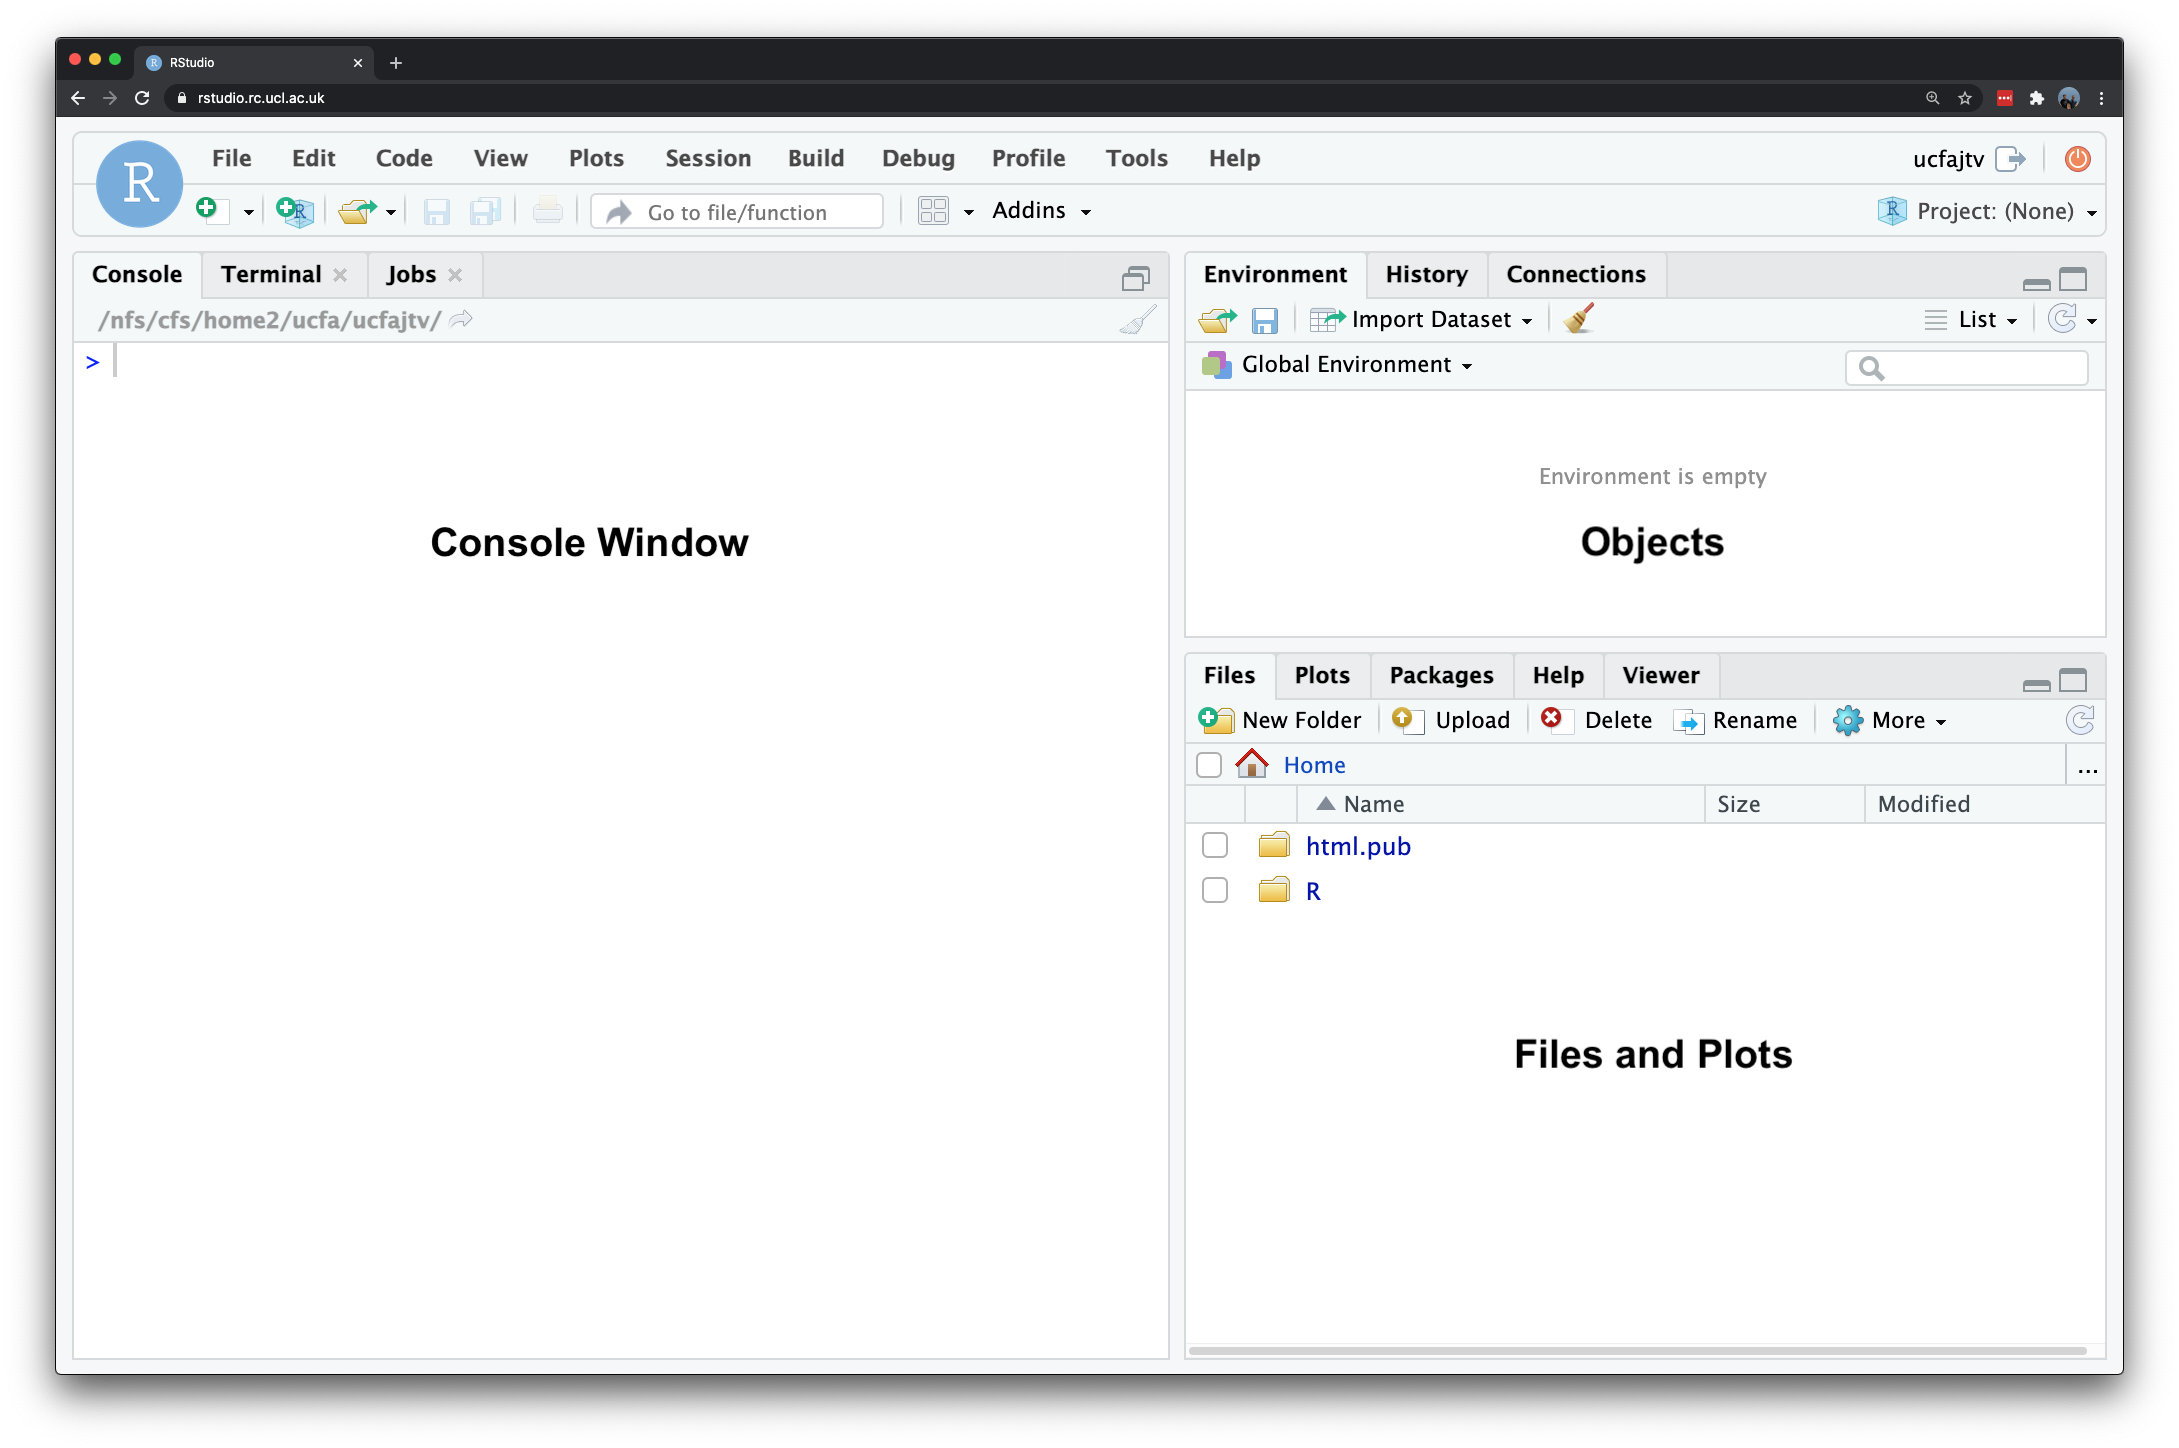
\includegraphics[width=30.26in]{images/w01/rstudio_interface} 

}

\caption{The RStudio Server interface.}\label{fig:01-rstudio-interface}
\end{figure}

\textbf{Note}
If it is the first time you log on to RStudio server you may only see the RStudio interface appear once you have clicked on the \emph{start a new session} button. More importantly: if you are not on campus, RStudio server will only work with an active Virtual Private Network (VPN) connection that links your personal computer into UCL's network. Details on setting up a VPN connection can be found in UCL's VPN connection guides: \href{https://www.ucl.ac.uk/isd/services/get-connected/ucl-virtual-private-network-vpn}{{[}Link{]}}

\hypertarget{r-package-installation}{%
\subsection{R package installation}\label{r-package-installation}}

Now we have installed or have access to QGIS and R, we need to customise R. Many useful R function come in packages, these are free libraries of code written and made available by other by R users. This includes packages specifically developed for data cleaning, data wrangling, visualisation, mapping, and spatial analysis. To save us some time, we will install all R packages that we will need over the next ten weeks in one go. Without going into detail on the RStudio (Server) interface, copy and paste the following code into the \emph{console}. You can execute the code by hitting \textbf{Enter}. This may take a while.

\begin{Shaded}
\begin{Highlighting}[]
\CommentTok{\# install all packages that we need}
\FunctionTok{install.packages}\NormalTok{(}\FunctionTok{c}\NormalTok{(}\StringTok{"tidyverse"}\NormalTok{, }\StringTok{"sf"}\NormalTok{, }\StringTok{"tmap"}\NormalTok{, }\StringTok{"osmdata"}\NormalTok{, }\StringTok{"RColorBrewer"}\NormalTok{, }\StringTok{"janitor"}\NormalTok{,}
    \StringTok{"spdep"}\NormalTok{, }\StringTok{"dbscan"}\NormalTok{, }\StringTok{"raster"}\NormalTok{, }\StringTok{"spatstat"}\NormalTok{, }\StringTok{"gstat"}\NormalTok{, }\StringTok{"dodgr"}\NormalTok{))}
\end{Highlighting}
\end{Shaded}

Once you have installed the packages, we need to check whether we can in fact load them into our R session. Copy and paste the following code into the \textbf{console}, and executed by hitting \textbf{Enter} again.

\begin{Shaded}
\begin{Highlighting}[]
\CommentTok{\# load all packages}
\FunctionTok{library}\NormalTok{(tidyverse)}
\FunctionTok{library}\NormalTok{(sf)}
\FunctionTok{library}\NormalTok{(tmap)}
\FunctionTok{library}\NormalTok{(osmdata)}
\FunctionTok{library}\NormalTok{(RColorBrewer)}
\FunctionTok{library}\NormalTok{(janitor)}
\FunctionTok{library}\NormalTok{(spdep)}
\FunctionTok{library}\NormalTok{(dbscan)}
\FunctionTok{library}\NormalTok{(raster)}
\FunctionTok{library}\NormalTok{(spatstat)}
\FunctionTok{library}\NormalTok{(gstat)}
\FunctionTok{library}\NormalTok{(dodgr)}
\end{Highlighting}
\end{Shaded}

You will see some information printed to your console but as long as you do not get a message that is similar to \texttt{Error:\ package\ or\ namespace\ load\ failed\ for\ \textless{}packagename\textgreater{}} or \texttt{Error:\ package\ \textquotesingle{}\textless{}packagename\textquotesingle{}\ could\ not\ be\ loaded} all should be fine.

\textbf{Note}
Even if you have used R or RStudio Server before and already installed some of the packages in the above list, do re-install all packages to make sure you have the latest versions. Legacy installations that have not been updated may lay lead to problems when going through the tutorials.

\hypertarget{a-note-on-arcgis}{%
\subsection{A note on ArcGIS}\label{a-note-on-arcgis}}

\href{https://www.esri.com/en-us/arcgis/products/arcgis-pro/overview}{ArcGIS Pro} (previously ArcMap) is the main commercial GIS software that you may have already used - or seen/heard about through other modules or even job adverts. We do not use ArcGIS Pro in our Practicals for several reasons:

\begin{itemize}
\tightlist
\item
  Computing requirements for ArcGIS Pro are substantial and it \textbf{only} operates on the Windows Operating System. For Mac users, using ArcGIS Pro (and ArcMap) would require using either a Virtual Machine or running a copy of Windows OS on a separate partition of your hard drive.
\item
  It is \textbf{proprietary} software, which means you need a license to use the software. For those of us in education, the University covers the cost of this license, but when you leave, you will need to pay for a personal license (around £100 for non-commercial use) to continue using the software and repeat any analysis you have used the software for.
\item
  Whilst ArcPro can use pure \href{https://www.python.org/}{Python} (and even R) as a programming language within it through scripts and notebooks, it primarily relies on its own \textbf{ArcPy} and \textbf{ArcGIS API for Python} packages to run the in-built tools and analytical functions. To use these packages, you still need a license which makes it difficult to share your code with others \emph{if} they do not have their own ArcGIS license.
\end{itemize}

Recent developments in the ArcPro software, however, does make it an attractive tool for spatial data science and quantitative geography - it has cross-user functionality, from data analysts who like to use a tool called Notebooks for their code development, to those focused more on cartography and visualisation with in-built bridges to Adobe's Creative Suite. We therefore do not want to put you off looking into ArcGIS in the future, but for this course, we want to ensure the reproducibility of your work.

\textbf{Note} This also means that the analysis you will be doing for your coursework assignment must be completed in R and QGIS. Specific guidance on the coursework assignment and permitted software will be made available at the end of Reading Week.

\hypertarget{byl-w01}{%
\section{Before you leave}\label{byl-w01}}

You should now be all ready to go with the computer practicals the coming week. \href{https://www.youtube.com/watch?v=d8Fmu3RLEOY}{That is it for this week}!

\hypertarget{giscience-and-gis-software}{%
\chapter{GIScience and GIS software}\label{giscience-and-gis-software}}

This week's lecture introduced you to foundational concepts associated with GIScience and GIS software, with particular emphasis on the representation of spatial data and sample design. Out of all our foundational concepts you will come across in the next four weeks, this is probably the most substantial to get to grips with and has both significant theoretical and practical aspects to its learning. The practical component of the week puts some of these learnings into practice, starting with a short digitisation excercise followed by a simple visualisation of London's population over time.

\hypertarget{reading-w02}{%
\section{Reading list}\label{reading-w02}}

\hypertarget{essential-readings-1}{%
\subsubsection*{Essential readings}\label{essential-readings-1}}
\addcontentsline{toc}{subsubsection}{Essential readings}

\begin{itemize}
\tightlist
\item
  Longley, P. \emph{et al.} 2015. Geographic Information Science \& Systems, \textbf{Chapter 2}: \emph{The Nature of Geographic Data}. \href{https://ucl.rl.talis.com/link?url=https\%3A\%2F\%2Fapp.knovel.com\%2Fhotlink\%2Ftoc\%2Fid\%3AkpGISSE001\%2Fgeographic-information-science\%3Fkpromoter\%3Dmarc\&sig=e437927b963cc591dcb65491eccdd3869cc31aef80e1443cb2ba12d8f3bb031a}{{[}Link{]}}
\item
  Longley, P. \emph{et al.} 2015. Geographic Information Science \& Systems, \textbf{Chapter 3}: \emph{Representing Geography}. \href{https://ucl.rl.talis.com/link?url=https\%3A\%2F\%2Fapp.knovel.com\%2Fhotlink\%2Ftoc\%2Fid\%3AkpGISSE001\%2Fgeographic-information-science\%3Fkpromoter\%3Dmarc\&sig=e437927b963cc591dcb65491eccdd3869cc31aef80e1443cb2ba12d8f3bb031a}{{[}Link{]}}
\item
  Longley, P. \emph{et al.} 2015. Geographic Information Science \& Systems, \textbf{Chapter 7}: \emph{Geographic Data Modeling}. \href{https://ucl.rl.talis.com/link?url=https\%3A\%2F\%2Fapp.knovel.com\%2Fhotlink\%2Ftoc\%2Fid\%3AkpGISSE001\%2Fgeographic-information-science\%3Fkpromoter\%3Dmarc\&sig=e437927b963cc591dcb65491eccdd3869cc31aef80e1443cb2ba12d8f3bb031a}{{[}Link{]}}
\end{itemize}

\hypertarget{suggested-readings-1}{%
\subsubsection*{Suggested readings}\label{suggested-readings-1}}
\addcontentsline{toc}{subsubsection}{Suggested readings}

\begin{itemize}
\tightlist
\item
  Goodchild, M. and Haining, R. 2005. GIS and spatial data analysis: Converging perspectives. \emph{Papers in Regional Science} 83(1): 363--385. \href{https://doi.org/10.1007/s10110-003-0190-y}{{[}Link{]}}
\item
  Schurr, C., Müller, M. and Imhof, N. 2020. Who makes geographical knowledge? The gender of Geography's gatekeepers. \emph{The Professional Geographer} 72(3): 317-331. \href{https://doi.org/10.1080/00330124.2020.1744169}{{[}Link{]}}
\item
  Yuan, M. 2001. Representing complex geographic phenomena in GIS. \emph{Cartography and Geographic Information Science} 28(2): 83-96. \href{https://doi.org/10.1559/152304001782173718}{{[}Link{]}}
\end{itemize}

\hypertarget{simple-digitisation-of-spatial-features}{%
\section{Simple digitisation of spatial features}\label{simple-digitisation-of-spatial-features}}

To get spatial features in a digital form, they need to be digitised. Let's take what should be a straight-forward example of digitising the River Thames in London.

\begin{figure}

{\centering 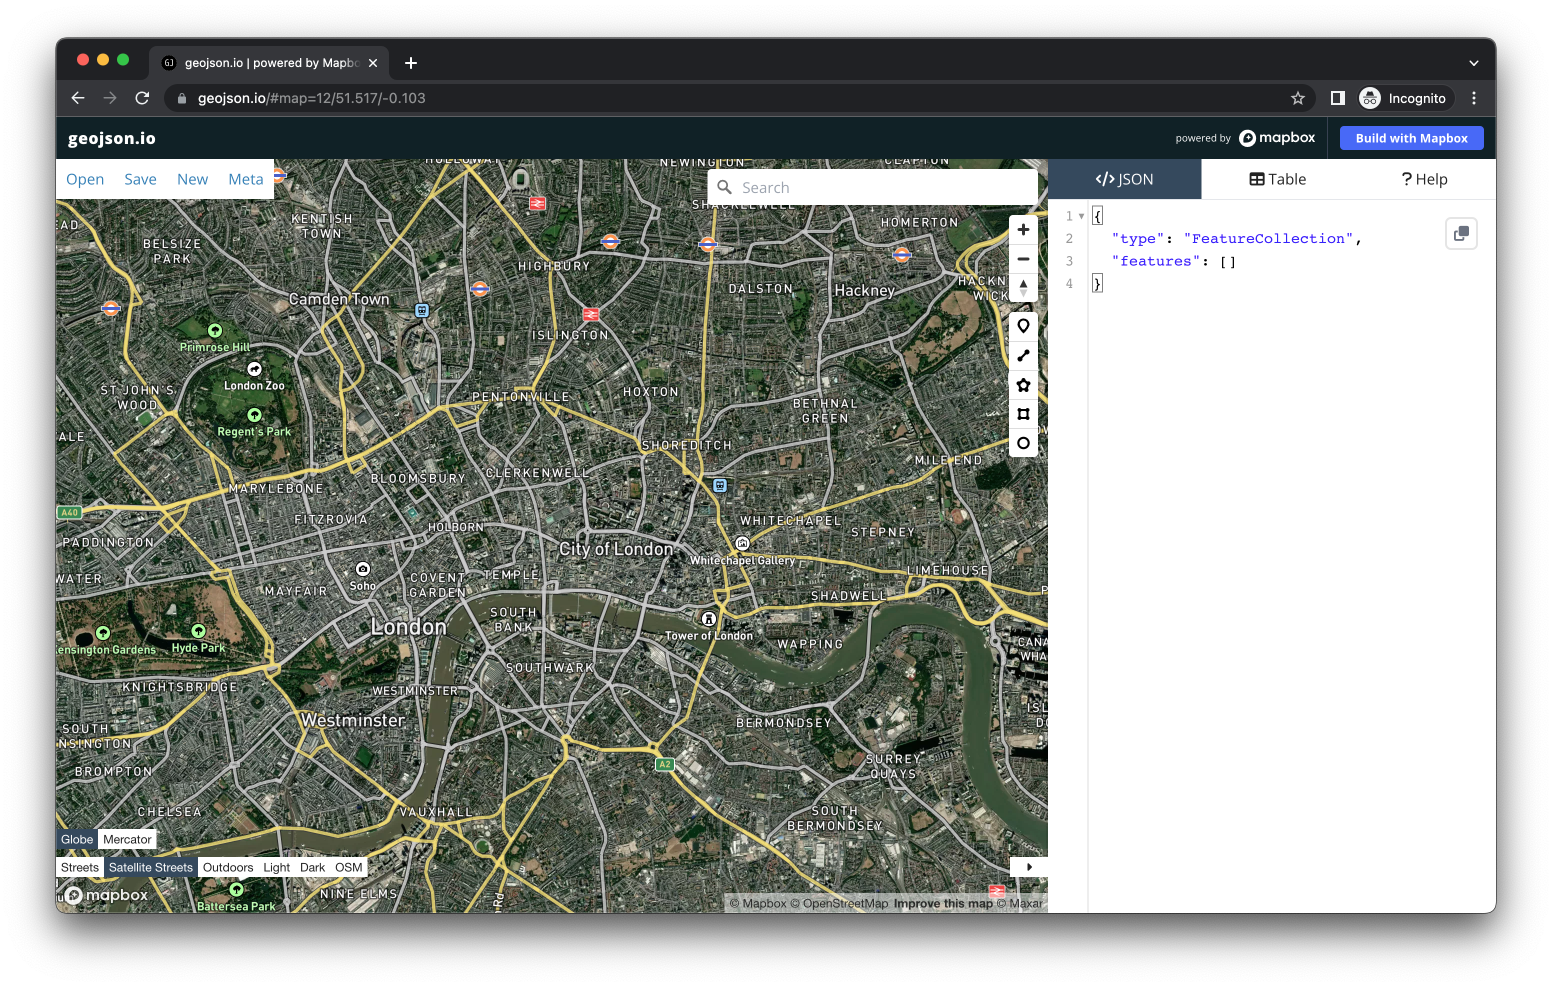
\includegraphics[width=0.9\linewidth]{images/w02/river_thames} 

}

\caption{The Thames.}\label{fig:02-digitise}
\end{figure}

We are going to use a very simple online tool that allows us to create digital data and export the data we create as raw files.

\begin{enumerate}
\def\labelenumi{\arabic{enumi}.}
\tightlist
\item
  Head to \href{http://geojson.io/\#map=12/51.5170/-0.1030}{geojson.io}.
\item
  In the bottom left-hand corner, select \emph{Satellite Streets} as your map option.
\item
  Next, click on the \texttt{Draw\ Linestring} tool which you can find on the right hand side of the screen. You can hover over the icons to get the names of each tool.
\item
  Now digitise the river Thames. Simply click from a starting point on the left- or right-hand side of the map, and digitise the river.
\item
  Once you are done, double-click your final point to end your line.
\item
  You can click on the line and select \emph{Info} in the pop-up screen to find out how long the line is.
\item
  You can export your data using the \emph{Save} menu.
\end{enumerate}

\hypertarget{questions}{%
\subsubsection*{Questions}\label{questions}}
\addcontentsline{toc}{subsubsection}{Questions}

\begin{itemize}
\tightlist
\item
  How easy did you find it to digitise the data and what decisions did you make in your own ``sample scheme''?
\item
  How close together are your clicks between lines?
\item
  Did you sacrifice detail over expediency or did you spend perhaps a little too long trying to capture ever small bend in the river?
\item
  How well do you think your line represents the River Thames?
\end{itemize}

\hypertarget{population-change-in-london}{%
\section{Population change in London}\label{population-change-in-london}}

The second part of this practical will introduces you to \textbf{attribute joins} followed by creating a \href{https://en.wikipedia.org/wiki/Choropleth_map}{choropleth map}. You will be using different types of \emph{joins} throughout this module, and probably the rest of your career, so it is incredibly important that you understand how they work.

\textbf{Note}
The datasets you will create in this practical will be used in next week's practical, so make sure to follow every step and save your data carefully.

When using spatial data, there is generally a very specific workflow that you will need to go through and, believe it or not, the majority of this is not actually focused on analysing your data. Along with the idea that 80\% of data is geographic data, the second most often-quoted GIS-related unreferenced `fact' is that anyone working with spatial data will spend 80\% of their time simply finding, retrieving, managing and processing the data before any analysis can be done.

One of the reasons behind this need for a substantial amount of processing is that the data you often need to use is almost never in the format that you require for analysis. For example, for our investigation, there is not a `ready-made' spatial population dataset (i.e.~population \texttt{shapefile}) we can download to explore population change across England:

\begin{figure}

{\centering 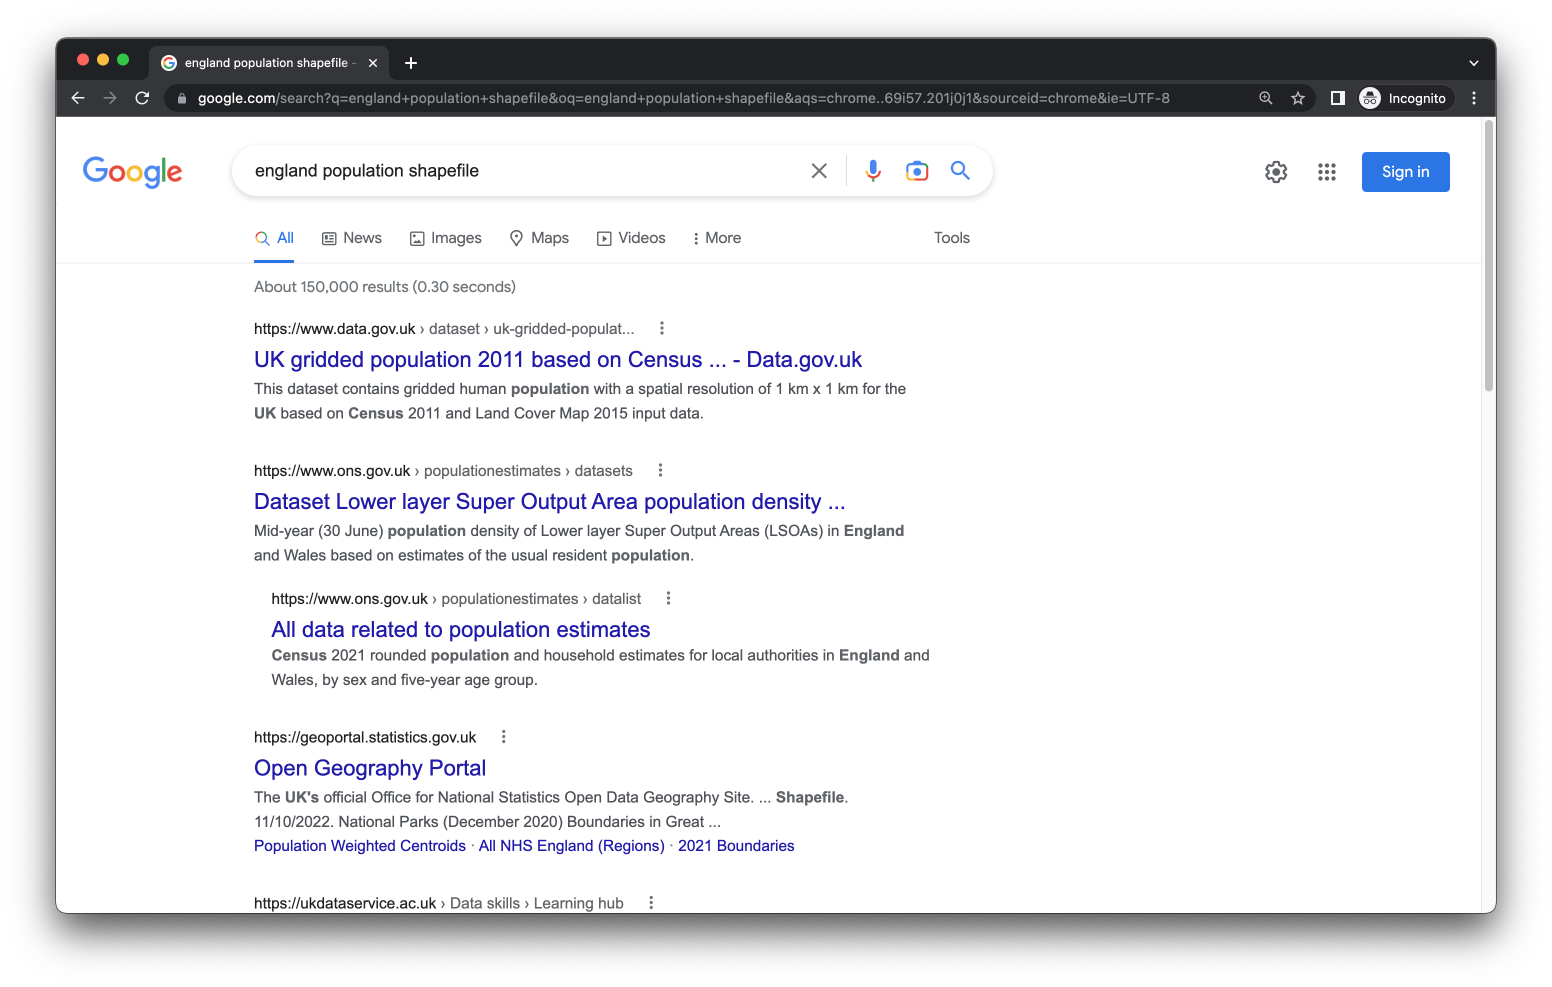
\includegraphics[width=0.9\linewidth]{images/w02/datasearch} 

}

\caption{Alas a quick Google search shows that finding a shapefile of England's population is not straightforward.}\label{fig:02-google-shp}
\end{figure}

Instead, we need to go and find the raw datasets and create the data layers that we want. As a result, before beginning any spatial analysis project, it is best-practice to think through what end product you will ultimately need for your analysis.

A typical spatial analysis workflow usually looks something like this:

\begin{itemize}
\tightlist
\item
  \textbf{Identify} the data you need to complete your analysis i.e.~answer your research questions. This includes thinking through the scale, coverage and currency of your dataset.
\item
  \textbf{Find} the data that matches your requirements, e.g.~is it openly and easily available?
\item
  \textbf{Download} the data and store it in the correct location.
\item
  \textbf{Clean} the data. This may be done before or after ingesting your data into your chosen software programme.
\item
  \textbf{Load} the data into your chosen software programme.
\item
  \textbf{Transform and process} the data. This may require re-projection, creating joins between datasets, calculating new fields and applying selections.
\item
  \textbf{Analyse} your data using appropriate methods.
\item
  \textbf{Visualise} your data and results with graphs and maps.
\item
  \textbf{Communicate} your results.
\end{itemize}

As you can see, the analysis and visualisation part comes quite late in the overall spatial analysis workflow - and instead, the workflow is very top-heavy with data management. However, very often in GIS-related courses you will be given pre-processed datasets. Because data management is an essential part of your workflow, we are clean (the majority of) our data from the get-go. This will help you understand the processes that you will need to go through in the future as you search for and download your own data, as well as deal with the data first-hand before loading it into our GIS software.

\hypertarget{w02-scene}{%
\subsection{Setting the scene}\label{w02-scene}}

For this practical, we will investigate how the population in London has changed over time. Understanding population change - over time and space - is spatial analysis at its most fundamental. We can understand a lot just from where population is growing or decreasing, including thinking through the impacts of these changes on the provision of housing, education, health and transport infrastructure.

We can also see first-hand the impact of wider socio-economic processes, such as urbanisation. Today we will look at population in London in 2011, 2015, and 2019 at the \emph{ward} scale that we can use within our future analysis projects, starting next week.

\textbf{Note}
We will use the population dataset to \emph{normalise} other datasets. Why? When we record events created by humans, there is often a population bias: simply, more people in an area will by probability lead to a higher occurrence of said event, such as crime. We will look at this in greater detail next week.

\hypertarget{w02-finding}{%
\subsection{Finding data}\label{w02-finding}}

In the UK, finding authoritative data on population and \emph{Administrative Geography} boundaries is increasingly straight-forward. Over the last decade, the UK government has opened up many of its datasets as part of an \textbf{Open Data} precedent that began in 2010 with the creation of \url{data.gov.uk} and the Open Government Licence (the terms and conditions for using data).

\href{www.data.gov.uk}{Data.gov.uk} is the UK government's central database that contains open data that the central government, local authorities and public bodies publish. This includes, for example, aggregated census and health data -- and even government spending. In addition to this central database, there are other authoritative databases run by the government and/or respective public bodies that contain either a specific type of data (e.g.~census data, crime data) or a specific collection of datasets (e.g.~health data from the NHS, data about London). Some portals are less up-to-date than others, so it is wise to double-check with the `originators' of the data to see if there are more recent versions.

For our practical, we will access data from two portals:

\begin{enumerate}
\def\labelenumi{\arabic{enumi}.}
\tightlist
\item
  For our administrative boundaries, we will download the \textbf{spatial} data from the \emph{London Datastore} (which is exactly what it sounds like).
\item
  For population, we will download \textbf{attribute} data from the \emph{Office of National Statistics (ONS)}.
\end{enumerate}

\hypertarget{w01-housekeeping}{%
\subsection{Housekeeping}\label{w01-housekeeping}}

Before we download our data, it is important to establish an organised file systems that we will use throughout the module:

\begin{enumerate}
\def\labelenumi{\arabic{enumi}.}
\tightlist
\item
  Create a \texttt{GEOG0030} folder in your \texttt{Documents} folder on your computer.
\item
  Within your \texttt{GEOG0030} folder, create the following subfolders:
\end{enumerate}

\begin{longtable}[]{@{}ll@{}}
\toprule()
Folder name & Purpose \\
\midrule()
\endhead
\texttt{data} & To store both raw data sets and final outputs. \\
\texttt{maps} & To save the maps you produce during your tutorials. \\
\bottomrule()
\end{longtable}

\begin{enumerate}
\def\labelenumi{\arabic{enumi}.}
\setcounter{enumi}{2}
\tightlist
\item
  Within your \texttt{data} folder, create the following subfolders:
\end{enumerate}

\begin{longtable}[]{@{}
  >{\raggedright\arraybackslash}p{(\columnwidth - 2\tabcolsep) * \real{0.2500}}
  >{\raggedright\arraybackslash}p{(\columnwidth - 2\tabcolsep) * \real{0.7500}}@{}}
\toprule()
\begin{minipage}[b]{\linewidth}\raggedright
Folder name
\end{minipage} & \begin{minipage}[b]{\linewidth}\raggedright
Purpose
\end{minipage} \\
\midrule()
\endhead
\texttt{raw} & To store all your raw data files that have not yet been processed. \\
\texttt{output} & To store all your final data files that have been processed and analysed, potentially ready to be mapped. \\
\bottomrule()
\end{longtable}

\hypertarget{w02-downloading}{%
\subsection{Downloading data}\label{w02-downloading}}

We will start by downloading the administrative geography boundaries:

\begin{enumerate}
\def\labelenumi{\arabic{enumi}.}
\tightlist
\item
  Navigate to the relevant page on the London Datastore: \href{https://data.london.gov.uk/dataset/statistical-gis-boundary-files-london}{{[}Link{]}}.
\item
  Download all three zipfiles to your computer: \texttt{statistical-gis-boundaries-london.zip}, \texttt{London-wards-2014.zip} and \texttt{London-wards-2018.zip}.
\end{enumerate}

The first dataset contains all levels of London's administrative boundaries. In descending size order: borough, Ward, Middle layer Super Output Area (MSOA), Lower layer Super Output Area (LSOA), and Output Area (OA) based on the 2011 Census. The second dataset contains an \emph{updated} version of the Ward boundaries, as of 2014. The third dataset contains yet another \emph{updated} version of the Ward boundaries, as of 2018. As we will be looking at population data for 2015 and 2019, it is best practice to use those boundaries that are most reflective of the `geography' at the time; therefore, we will use these 2014 / 2018 ward boundaries for our 2015 / 2019 population dataset, respectively.

\textbf{Note}
Once downloaded, you will need to unzip all files before you can use them. To unzip the file, you can use the built-in functionality of your computer's operating system. For Windows: right click on the zip file, select \textbf{Extract All}, and then follow the instructions. For Mac OS: double-click on the the zip file and it should unzip automatically.

Once unzipped, you will find two folders: \emph{Esri} and \emph{MapInfo.} These folders contain the same data but in different data formats: \textbf{Esri shapefile} and \textbf{MapInfo TAB}.

\textbf{Note}
MapInfo is another proprietary GIS software, which has historically been used in public sectors services in the UK and abroad, although has generally been replaced by either Esri's ecosystem or open-source software GIS.

Now open your \texttt{GEOG0030/data/raw/} folder and create a new folder called \texttt{boundaries}. Within this folder, create three new folders: \texttt{2011}, \texttt{2014} and \texttt{2018}. Copy the entire contents of \texttt{Esri} folder of each year into their respective year folder.

We do not want to add the additional \texttt{Esri} folder as a step in our filesystem, i.e.~your file paths should read: \texttt{GEOG0030/data/raw/boundaries/2011} for the 2011 boundaries, \texttt{GEOG0030/data/raw/boundaries/2014} for the 2014 boundaries, and \texttt{GEOG0030/data/raw/boundaries/2018} for the 2018 boundaries.

\begin{figure}

{\centering 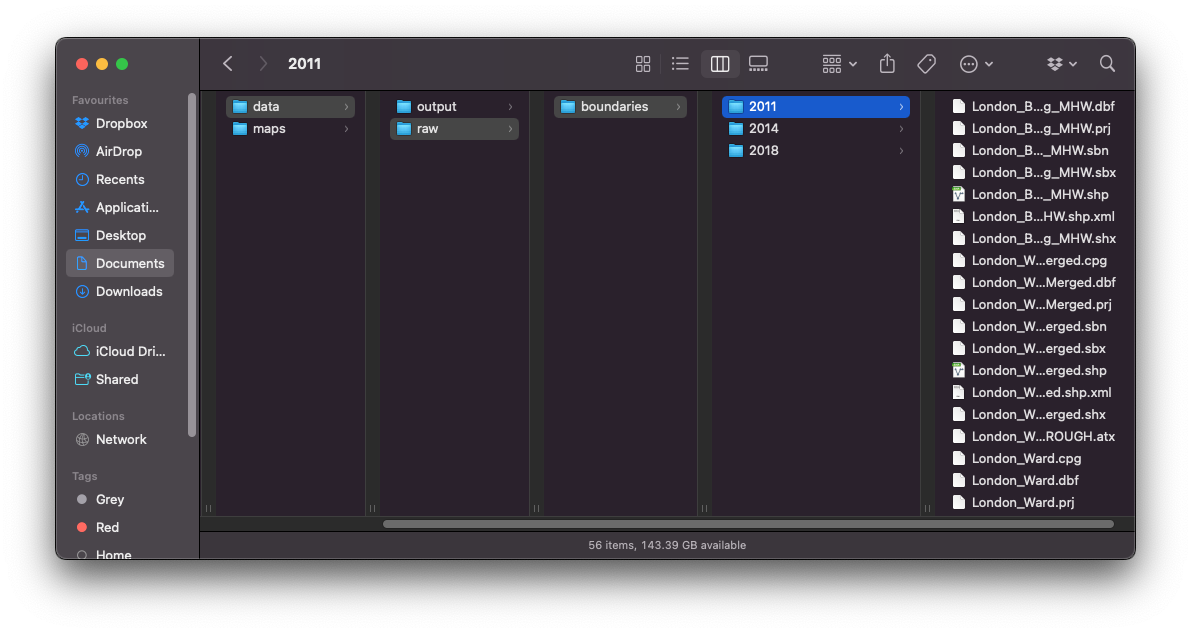
\includegraphics[width=0.9\linewidth]{images/w02/file_management} 

}

\caption{Your setup should look something like this.}\label{fig:02-setup}
\end{figure}

We now have our administrative geography files ready for use.

\textbf{Note}
Administrative geographies are a way of dividing the country into smaller sub-divisions or areas that correspond with the area of responsibility of local authorities and government bodies. These administrative sub-divisions and their associated geography have several important uses, including assigning electoral constituencies, defining jurisdiction of courts, planning public healthcare provision, as well as what we are concerned with: used as a mechanism for collecting census data and assigning the resulting datasets to a specific administrative unit. These geographies are updated as populations evolve and as a result, the boundaries of the administrative geographies are subject to either periodic or occasional change. The UK has quite a complex administrative geography, particularly due to having several countries within one overriding administration and then multiple ways of dividing the countries according to specific applications. More details on the administrative geographies of the UK can be found on the website of the \href{https://www.ons.gov.uk/methodology/geography/ukgeographies/administrativegeography}{Office for National Statistics}.

For our population datasets, we will use the ONS mid-year estimates (MYE). These population datasets are estimates that are based on the 2011 census count and then updated with estimated population growth. They are released once a year, with a delay of a year. Today we will use the data for 2011, 2015, and 2019.

\begin{enumerate}
\def\labelenumi{\arabic{enumi}.}
\tightlist
\item
  Navigate to the \emph{ward} level datasets: \href{https://www.ons.gov.uk/peoplepopulationandcommunity/populationandmigration/populationestimates/datasets/wardlevelmidyearpopulationestimatesexperimental}{{[}Link{]}}
\item
  When you navigate to this page, you will find multiple choices of data to download. We will need to download the estimates for \textbf{2011, 2015} and \textbf{2019}. Click to download each of the zipfiles. Choose the \textbf{revised} versions for 2015 and the (Census-based) 2011 wards edition for 2011.
\item
  In your \texttt{GEOG0030/data/raw/} folder, create a new folder called \texttt{population}, unzip your downloaded files, and copy the three spreadsheets to the newly created \texttt{population} folder.
\item
  Rename the files you donwloaded to: \texttt{MYE\_ward\_2011.xls}, \texttt{MYE\_ward\_2015.xls}, and \texttt{MYE\_ward\_2019.xlsx}.
\end{enumerate}

Now it is time to do some quite extensive data cleaning and preparation.

\hypertarget{w02-cleaning}{%
\subsection{Cleaning data}\label{w02-cleaning}}

When you open up any of the ward spreadsheets in Excel =, you will notice that there are several worksheets contained in this workbook. However, we are only interested in the total population tab. We therefore need to copy over the data from the 2011, 2015 and 2019 datasets into separate \texttt{csv} files.

\hypertarget{london-population-in-2011}{%
\subsubsection{London population in 2011}\label{london-population-in-2011}}

\begin{enumerate}
\def\labelenumi{\arabic{enumi}.}
\tightlist
\item
  Open the 2011 ward spreadsheet in Excel.
\item
  Click on the \texttt{Mid-2011\ Persons} tab and have a look at the data. As you should be able to see, we have a set of different fields (e.g.~\texttt{Ward\ Code}, \texttt{Ward\ Name}), including population counts. Because we do not need all the data in the spreadsheet, we will extract only the data we need for our analysis. This means we need the total population (\texttt{All\ Ages}) data, alongside some identifying information that distinguishes each record from one another. Here we can see that both \texttt{Ward\ Code} and \texttt{Ward\ Name} suit this requirement. We can also think that the \texttt{Local\ Authority} column might be of use, so we also keep this information.
\item
  Create a new Excel spreadsheet Excel and from the \texttt{Mid-2011\ Persons} spreadsheet, copy over all cells from columns \textbf{A} to \textbf{D} and rows \textbf{4 to 636} into this new spreadsheet. Row 636 denotes the end of the \emph{Greater London} wards (i.e.~the end of the \emph{Westminster Local Authority}) which are kept (in most scenarios) at the top of the spreadsheet as their \textbf{Ward Codes} are the first in sequential order.
\item
  Before we go any further, we need to format our data. First, we want to rename our fields to remove the spaces and superscript formatting. Re-title the fields as follows: \texttt{ward\_code}, \texttt{ward\_name}, \texttt{local\_authority} and \texttt{pop2011}.
\item
  One further bit of formatting that you must do before saving your data is to format our population field. At the moment, you will see that there are commas separating the thousands within our values. If we leave these commas in our values, QGIS will read them as decimal points, creating decimal values of our population. There are many points at which we could solve this issue, but the easiest point is now - we will strip our population values of the commas and set them to integer (whole numbers) values. To format the \texttt{pop2011} column, select the entire column and right-click on the \texttt{D} cell. Click on \textbf{Format Cells} and set the Cells to \textbf{Number} with \textbf{0} decimal places. You should see that the commas are now removed from your population values.
\item
  Save your spreadsheet into your \texttt{output} folder as \texttt{ward\_population\_2011.csv}.
\end{enumerate}

\hypertarget{london-population-in-2015}{%
\subsubsection{London population in 2015}\label{london-population-in-2015}}

\begin{enumerate}
\def\labelenumi{\arabic{enumi}.}
\tightlist
\item
  Open the 2015 ward spreadsheet in Excel.
\item
  As you will see again, there are plenty of worksheets available and we want to select the \texttt{Mid-2015\ Persons} tab. We now need to copy over the data from our 2015 dataset to a new spreadsheet again. However, at first instance, you will notice that the City of London (CoL) wards are missing from this dataset. Then if you scroll to the end of the London Local Authorities, i.e.~to the bottom of Westminster, what you should notice is that the final row for the Westminster data is in fact row 575 - this suggests we are missing the data fror some Local Authorities (LAs). We need to determine which ones are missing and try to find them in the 2015 spreadsheet. With this in mind, start by copying over all cells from columns \textbf{A} to \textbf{D} and rows \textbf{5 to 575} into a new spreadsheet.
\item
  If you were to compare the names of the London Boroughs that we have now copied with the full list, you would notice that we are missing \emph{City of London}, \emph{Hackney}, \emph{Kensington and Chelsea}, and \emph{Tower Hamlets}. If we head back to the original 2015 raw dataset, we can actually find this data (as well as the City of London) further down in the spreadsheet. It seems like these LAs had their codes revised in the 2014 revision and are no longer in the same order as the 2011 dataset.
\item
  Locate the data for the \emph{City of London}, \emph{Hackney}, \emph{Kensington and Chelsea} and \emph{Tower Hamlets} and copy this over into our new spreadsheet. Double-check that you now have in total \textbf{637} wards within your dataset.
\item
  Remember to rename the fields as above, but change your population field to \textbf{pop2015}. Also, remember to reformat the values in your \texttt{pop2015} column.
\item
  Once complete, save your spreadsheet into your \texttt{output} folder as \texttt{ward\_population\_2015.csv}.
\end{enumerate}

\hypertarget{london-population-in-2019}{%
\subsubsection{London population in 2019}\label{london-population-in-2019}}

\begin{enumerate}
\def\labelenumi{\arabic{enumi}.}
\tightlist
\item
  Open the 2019 ward spreadsheet in Excel. This time we are interested in the \texttt{Mid-2019\ Persons} tab.
\item
  This time the data that we are interested in can be found in columns \texttt{A}, \texttt{B}, \texttt{D} and \texttt{G}. Because the columns that we want are not positioned next to one antoher, start by hiding columns \texttt{C}, \texttt{E} and \texttt{F}. You can do this by right-clicking on the colums you want to hide and selecting \textbf{Hide}.
\item
  Next, copy the data from \textbf{row 5 to the final row for the Westminster data} for columns \texttt{A}, \texttt{B}, \texttt{D} and \texttt{G} over into a new spreadsheet.
\item
  If you look at the total rows that we have copied over, we have even fewer wards than the 2015 dataset. This time we are not only missing data for \emph{City of London}, \emph{Hackney}, \emph{Kensington and Chelsea}, \emph{Tower Hamlets} but also for \emph{Bexley}, \emph{Croydon}, \emph{Redbridge}, and \emph{Southwark}.
\item
  Copy over the remaining wards for these Local Authorities/boroughs.
\item
  Once you've copied them over - you should now have \textbf{640} wards. Delete columns \texttt{C}, \texttt{E} and \texttt{F} and rename the remaining fields as you have done previously. Also, remember to reformat the values in your \texttt{pop2019} column.
\item
  Once complete, save your spreadsheet into your \texttt{output} folder as \texttt{ward\_population\_2019.csv}.
\end{enumerate}

You should now have your three population \texttt{csv} datasets in your \texttt{output} folder. We are now (finally) ready to start using our data within QGIS.

\hypertarget{using-qgis-to-map-our-population-data}{%
\subsection{Using QGIS to map our population data}\label{using-qgis-to-map-our-population-data}}

\hypertarget{setting-up-a-project}{%
\subsubsection{Setting up a project}\label{setting-up-a-project}}

We will now use QGIS to create population maps for the wards in London across our three time periods. To achieve this, we need to \textbf{join our table data to our spatial datasets} and then map our populations for our visual analysis.

Because, as we have seen above, we have issues with the number of wards and changes in boundaries across our three years, we will not (for now) complete any quantitative analysis of these population changes - this would require significant additional processing that we do not have time for today.

\textbf{Note}
Data interoperability is a key issue that you will face in spatial analysis, particularly when it comes to Administrative Geographies.

\begin{enumerate}
\def\labelenumi{\arabic{enumi}.}
\tightlist
\item
  Start \textbf{QGIS}.
  Let's start a new project.
\item
  Click on \textbf{Project} -\textgreater{} \textbf{New}. Save your project into your \texttt{qgis} folder as \texttt{w2-pop-analysis}. Remember to save your work throughout the practical.
\item
  Before we get started with adding data, we will first set the Coordinate Reference System of our Project. Click on \textbf{Project} -\textgreater{} \textbf{Properties -- CRS}. In the Filter box, type \textbf{British National Grid}. Select \textbf{OSGB 1936 / British National Grid - EPSG:27700} and click Apply. Click \textbf{OK}.
\end{enumerate}

\textbf{Note}
We will explain CRSs and using CRSs in GIS software in more detail next week.

\hypertarget{adding-layers}{%
\subsubsection{Adding layers}\label{adding-layers}}

We will first focus on loading and joining the 2011 datasets.

\begin{enumerate}
\def\labelenumi{\arabic{enumi}.}
\setcounter{enumi}{4}
\item
  Click on \textbf{Layer} -\textgreater{} \textbf{Add Layer} -\textgreater{} \textbf{Add Vector Layer}.
\item
  With \textbf{File} select as your source type, click on the small three dots button and navigate to your 2011 boundary files.
\item
  Here, we will select the \texttt{London\_Ward.shp} dataset. Click on the \texttt{.shp} file of this dataset and click \textbf{Open}. Then click \textbf{Add}. You may need to close the box after adding the layer.
\end{enumerate}

We can take a moment just to look at our ward data - and recognise the shape of London. Can you see the City of London in the dataset? It has the smallest wards in the entire London area. With the dataset loaded, we can now explore it in a little more detail. We want to check out two things about our data: first, its \textbf{Properties} and secondly, its \textbf{Attribute Table}.

\begin{enumerate}
\def\labelenumi{\arabic{enumi}.}
\setcounter{enumi}{7}
\tightlist
\item
  Right-click on the \texttt{London\_Ward} layer and open the \textbf{Attribute Table} and look at how the attributes are stored and presented in the table. Explore the different buttons in the Attribute Table and see if you can figure out what they mean. Once done, close the Attribute Table.
\item
  Right-click on the \texttt{London\_Ward} layer and select \textbf{Properties}. Click through the different tabs and see what they contain. Keep the \textbf{Properties} box open.
\end{enumerate}

Before adding our population data, we can make a quick map of the wards in London - we can add labels and change the \emph{symbolisation} of our wards.

\begin{enumerate}
\def\labelenumi{\arabic{enumi}.}
\setcounter{enumi}{9}
\item
  In the \textbf{Properties} box, click on the \textbf{Symbology} tab - this is where we can change how our data layer looks. For example, here we can change the line and fill colour of our wards utilising either the default options available or clicking on \textbf{Simple Fill} and changing these properties directly. Keep the overall \textbf{styling} to a \textbf{Single Symbol} for now - we will get back to this once we have added the population data. You can also click on the \textbf{Labels} tab - and set the Labels option to \textbf{Single labels}.
\item
  QGIS will default to the \textbf{NAME} column within our data. You can change the properties of these labels using the options available. Change the font to \textbf{Futura} and size \textbf{8} and under the add a small buffer to the labels by selecting \textbf{Draw text bufer} under the \textbf{Buffer} tab. You can click \textbf{Apply} to see what your labels look like. Please note that the background colour may differ.
\end{enumerate}

\begin{figure}

{\centering 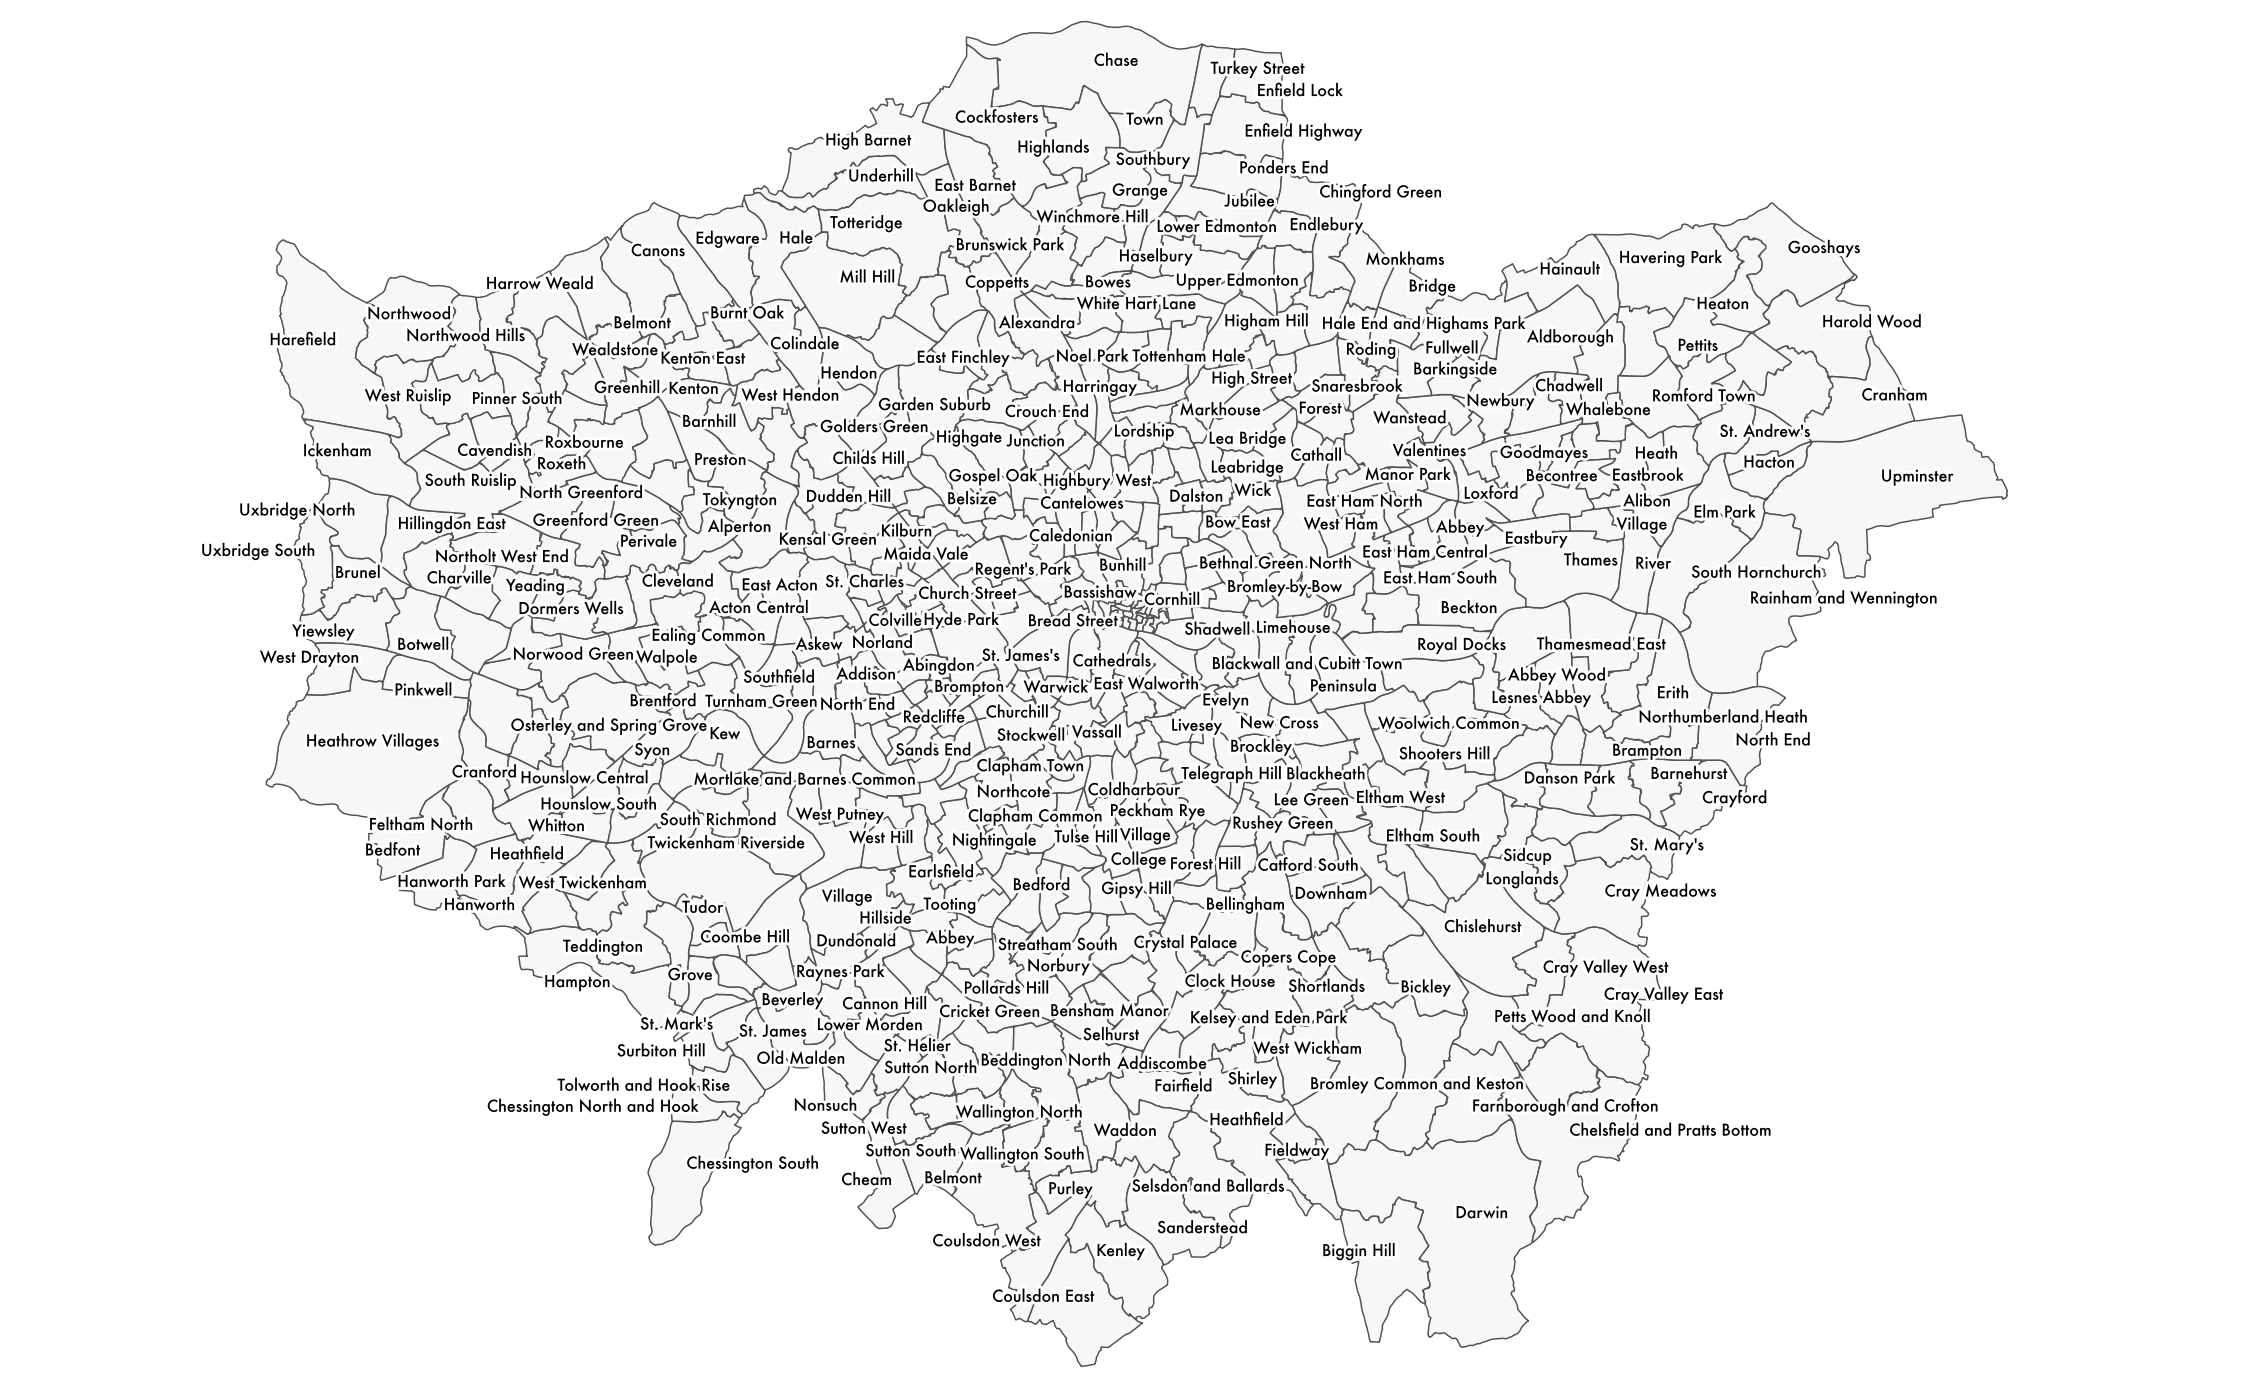
\includegraphics[width=31.31in]{images/w02/wardlabels} 

}

\caption{It looks incredibly busy.}\label{fig:02-busy-labels}
\end{figure}

\begin{enumerate}
\def\labelenumi{\arabic{enumi}.}
\setcounter{enumi}{11}
\tightlist
\item
  Click \textbf{OK} once you are done changing the Symbology and Label style of your data to return to the main window.
\end{enumerate}

\textbf{Note}
The main strength of a GUI GIS system is that is really helps us understand how we can visualise spatial data. Even with just these two shapefiles loaded, we can understand two key concepts of using spatial data within GIS.

The first, and this is only really relevant to GUI GIS systems, is that each layer can either be turned on or off, to make it visible or not (try clicking the tick box to the left of each layer). This is probably a feature you are used to working with if you have played with interactive web mapping applications before!

The second concept is the order in which your layers are drawn -- and this is relevant for both GUI GIS and when using plotting libraries such as \texttt{ggplot2} or \texttt{tmap} in RStudio. Your layers will be drawn depending on the order in which your layers are either tabled (as in a GUI GIS) or `called' in your function in code.

Being aware of this need for `order' is important when we shift to using RStudio and \texttt{tmap} to plot our maps, as if you do not layer your data correctly in your code, your map will end up not looking as you hoped!

For us using QGIS right now, the layers will be drawn from bottom to top. At the moment, we only have one layer loaded, so we do not need to worry about our order right now - but as we add in our 2015 and 2018 ward files, it is useful to know about this order as we will need to display them individually to export them at the end.

\hypertarget{conducting-an-attribute-join}{%
\subsubsection{Conducting an attribute join}\label{conducting-an-attribute-join}}

We are now going to join our 2011 population data to our 2011 shapefile. First, we need to add the 2011 population data to our project.

\begin{enumerate}
\def\labelenumi{\arabic{enumi}.}
\setcounter{enumi}{12}
\item
  Click on \textbf{Layer} -\textgreater{} \textbf{Add Layer} -\textgreater{} \textbf{Add Delimited Text Layer}.
\item
  Click on the three dots button again and navigate to your \textbf{2011 population data} in your \texttt{working} folder. Your file format should be set to \texttt{csv}. You should have the following boxes clicked under the \textbf{Record and Field options} menu: \emph{Decimal separator is comma; First record has field names; Detect field types; Discard empty fields}. QGIS does many of these by default, but do double-check!
\item
  Set the Geometry to \emph{No geometry (attribute only table)} under the \textbf{Geometry Definition} menu. Then click \textbf{Add} and \textbf{Close}. You should now see a table added to your \texttt{Layers} box.
\end{enumerate}

We can now join this table data to our spatial data using an \textbf{Attribute Join}.

\textbf{Note}
An attribute join is one of two types of data joins you will use in spatial analysis (the other is a spatial join, which we will look at later on in the module). An attribute join essentially allows you to join two datasets together, as long as they share a common attribute to facilitate the `matching' of rows:

\begin{center}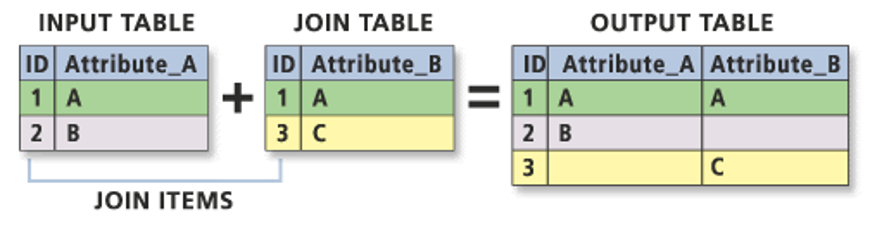
\includegraphics[width=12.08in]{images/w02/attribute_joins} \end{center}

Essentially you need a \textbf{single identifying ID} field for your records within both datasets: this can be a code, a name or any other string of information. In spatial analysis, we always \textbf{join our table data to our shape data} (One way to think about it as attaching the table data to each shape).

As a result, your target layer is always the shapefile (or spatial data) whereas your join layer is the table data. These are known as the left- and right-side tables when working with code.

\textbf{To make a join work, you need to make sure your ID field is correct across both datasets}, i.e.~no typos or spelling mistakes. Computers can only follow instructions, so they do not know that \emph{St.~Thomas} in one dataset is that same as \emph{St Thomas} in another, or even \emph{Saint Thomas}! It will be looking for an exact match!

As a result, whilst in our datasets we have kept both the name and code for both the boundary data and the population data, \textbf{when creating the join, we will always prefer to use the CODE over their names}. Unlike names, codes reduce the likelihood of error and mismatch because they do not rely on understanding spelling!

Common errors, such as adding in spaces or using \texttt{0} instead \texttt{O} (and vice versa) can still happen -- but it is less likely.

To make our join work, we need to check that we have a matching \textbf{UID} across both our datasets. We therefore need to look at the tables of both datasets and check what attributes we have that could be used for this possible match.

\begin{enumerate}
\def\labelenumi{\arabic{enumi}.}
\setcounter{enumi}{15}
\item
  Open up the Attribute Tables of each layer and check what fields we have that could be used for the join. We can see that both our respective ``code'' fields have the same codes (\texttt{ward\_code} and \texttt{GSS\_code}) so we can use these to create our joins.
\item
  Right-click on your \texttt{London\_Ward} layer -\textgreater{} \textbf{Properties} and then click on the \textbf{Joins} tab.
\end{enumerate}

\begin{itemize}
\tightlist
\item
  Click on the \textbf{+} button. Make sure the \textbf{Join Layer} is set to \texttt{ward\_population\_2011}.
\item
  Set the \textbf{Join field} to \texttt{ward\_code}.
\item
  Set the \textbf{Target field} to \texttt{GSS\_code}.
\item
  Click the \textbf{Joined Fields} box and click to only select the \texttt{pop2011} field.
\item
  Click on the \textbf{Custom Field Name Prefix} and \textbf{remove} the pre-entered text to leave it blank.
\item
  Click on \textbf{OK}.
\item
  Click on \textbf{Apply} in the main Join tab and then click \textbf{OK} to return to the main QGIS window.
\end{itemize}

We can now check to see if our join has worked by opening up our \texttt{London\_Ward} \textbf{Attribute Table} and looking to see if our wards now have a \textbf{Population} field attached to it.

\begin{enumerate}
\def\labelenumi{\arabic{enumi}.}
\setcounter{enumi}{17}
\tightlist
\item
  Right-click on the \texttt{London\_Ward} layer and open the \textbf{Attribute Table} and check that the population data column has been added to the table.
\end{enumerate}

As long as it has joined, you can move forward with the next steps. If your join has not worked, try the steps again - and if you are still struggling, do let us know.

\textbf{Note}
Now, the join that you have created between your ward and population datasets in only held in QGIS's memory. If you were to close the programme now, you would lose this join and have to repeat it the next time you opened QGIS. To prevent this from happening, we need to export our dataset to a new shapefile - and then re-add this to the map.

Let's do this now:

\begin{enumerate}
\def\labelenumi{\arabic{enumi}.}
\setcounter{enumi}{18}
\tightlist
\item
  Right-click on your \texttt{London\_Ward} shapefile and click \textbf{Export} -\textgreater{} \textbf{Save Features As\ldots{}}. The format should be set to an ESRI shapefile.
\end{enumerate}

\begin{itemize}
\tightlist
\item
  Then click on the three dots buttons and navigate to your \texttt{final} folder and enter: \texttt{ward\_population\_2011} as your file name.
\item
  Check that the \textbf{CRS} is \textbf{British National Grid}.
\item
  Leave the remaining fields as selected, but check that the \textbf{Add saved file to map} is checked. Click \textbf{OK}.
\end{itemize}

You should now see our new shapefile add itself to our map. You can now remove the original \texttt{London\_Ward} and \texttt{ward\_population\_2011} datasets from our Layers box (Right-click on the layers and opt for \textbf{Remove Layer\ldots{}}).

The final thing we would like to do with this dataset is to style our dataset by our newly added population field to show population distribution around London.

\begin{enumerate}
\def\labelenumi{\arabic{enumi}.}
\setcounter{enumi}{19}
\tightlist
\item
  To do this, again right-click on the \textbf{Layer} -\textgreater{} \textbf{Properties} -\textgreater{} \textbf{Symbology}.
\end{enumerate}

\begin{itemize}
\tightlist
\item
  This time, we want to style our data using a \textbf{Graduated} symbology.
\item
  Change this option in the tab and then choose \texttt{pop2011} as your column.
\item
  We can then change the color ramp to suit our aesthetic preferences - \emph{Viridis} seems to be the cool colour scheme at the moment, and we will choose to invert our ramp as well.
\item
  The final thing we need to do is \textbf{classify} our data - what this simply means is to decide how to group the values in our dataset together to create the graduated representation.
\item
  We will be looking at this in later weeks, but for now, we will use the \textbf{Natural Breaks} option.
\item
  Click on the drop-down next to Mode, select \textbf{Natural Breaks}, change it to \textbf{7} classes and then click \textbf{Classify}.
\item
  Finally click \textbf{Apply} to style your dataset.
\end{itemize}

\textbf{Note}
Understanding what classification is appropriate to visualise your data is an important step within spatial analysis and visualisation, and something you will learn more about in the following weeks. Overall, they should be determined by understanding your data's distribution and match your visualisation accordingly.

Feel free to explore using the different options with your dataset at the moment -- the results are almost instantaneous using QGIS, which makes it a good playground to see how certain parameters or settings can change your output.

You should now be looking at something like this:

\begin{figure}

{\centering 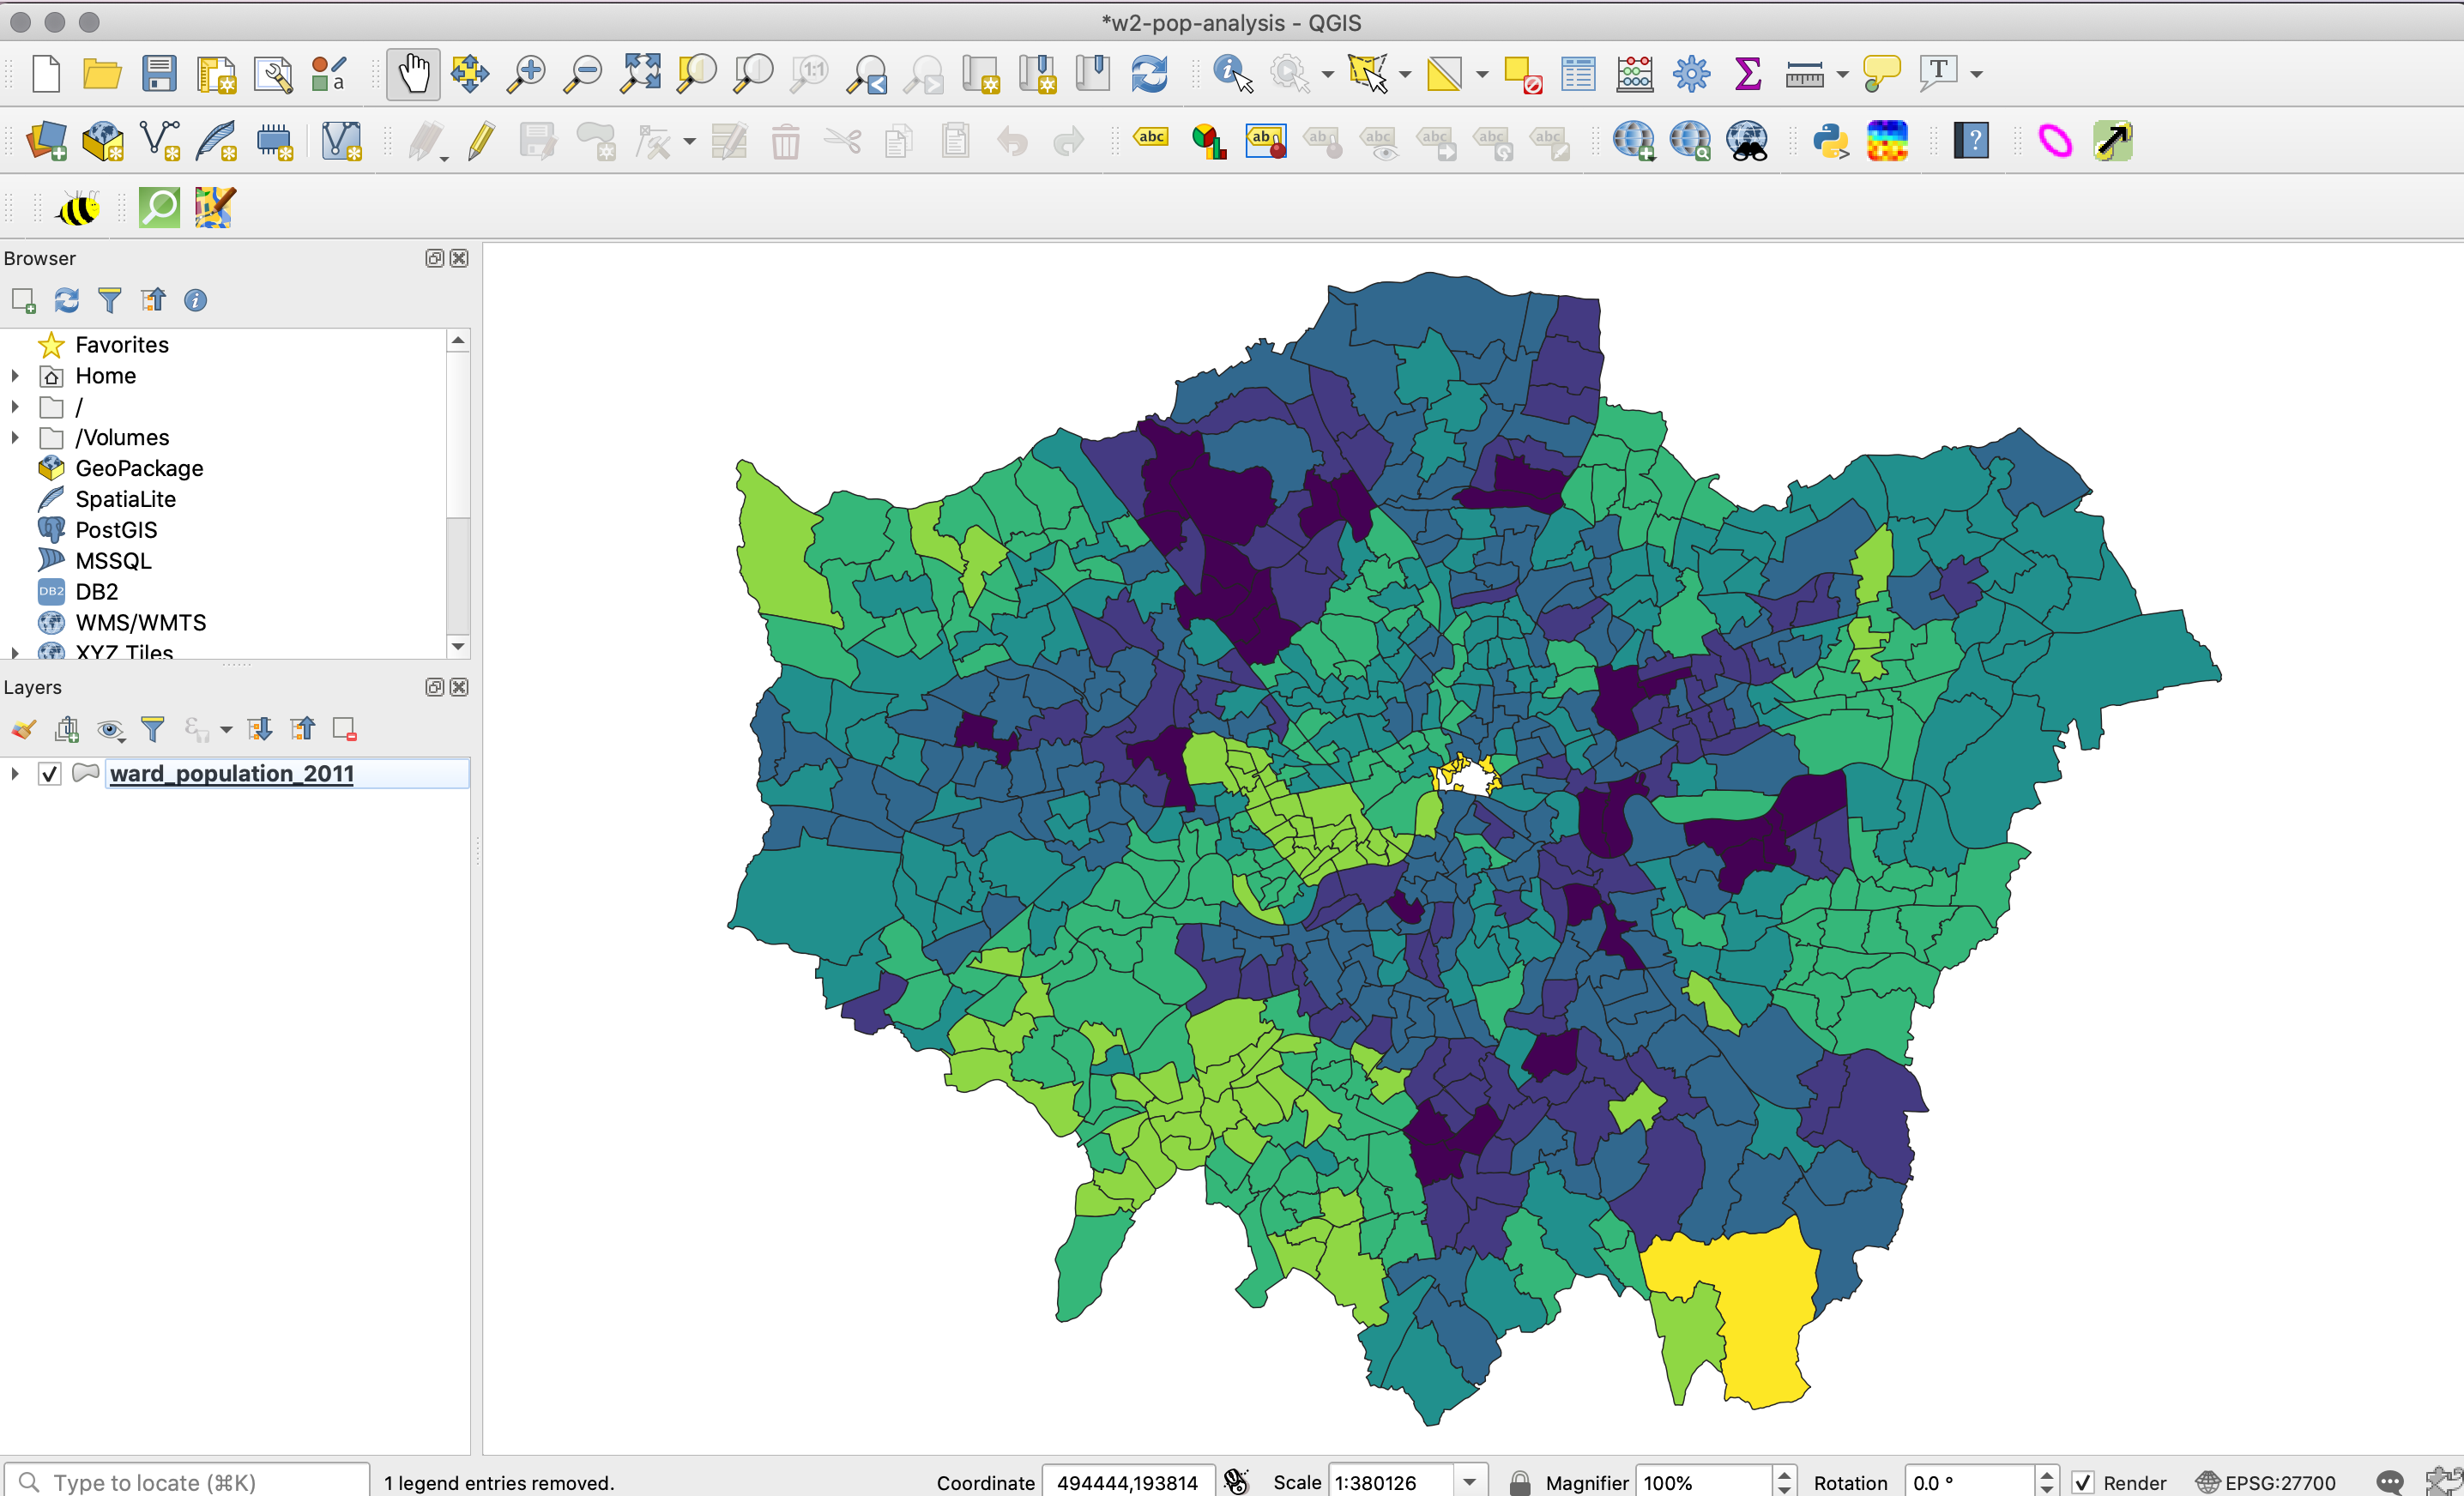
\includegraphics[width=39.89in]{images/w02/ward_2011} 

}

\caption{Your result.}\label{fig:02-ward-result}
\end{figure}

You will be able to see that we have \textbf{some} missing data - and this is for several wards within the City of London. This is because census data is \textbf{only recorded for 8 out of the 25 wards} and therefore we have no data for the remaining wards. As a result, these wards are left blank, i.e.~white, to represent a \texttt{NODATA} value.

One thing to flag is that \texttt{NODATA} means no data - whereas \texttt{0}, particularly in a scenario like this, would be an actual numeric value. It is important to remember this when processing and visualising data, to make sure you do not represent a \texttt{NODATA} value incorrectly.

\hypertarget{exporting-map-for-visual-analysis}{%
\subsection{Exporting map for visual analysis}\label{exporting-map-for-visual-analysis}}

To export your map (as is):
- Select only the map layers you want to export and then opt for \textbf{Project} -\textgreater{} \textbf{Import/Export} -\textgreater{} \textbf{Export to Image} and save your final map in your \texttt{maps} folder. You may want to create a folder for these maps titled \texttt{w02}.

Next week, we will look at how to style our maps using the main map conventions (adding North Arrows, Scale Bars and Legends) but for now a simple picture will do.

\hypertarget{assignment-w02}{%
\section{Assignment}\label{assignment-w02}}

You now need to \textbf{repeat this whole process} for your 2015 and 2019 datasets. Remember, you need to:

\begin{itemize}
\tightlist
\item
  Load the respective Ward dataset as a Vector Layer.
\item
  Load the respective Population dataset as a Delimited Text File Layer (remember the settings!).
\item
  Join the two datasets together using the Join tool in the Ward dataset Properties box.
\item
  Export your joined dataset into a new dataset within your \texttt{final} folder.
\item
  Style your data appropriately.
\item
  Export your maps as an image to your \texttt{maps} folder.
\end{itemize}

To make visual comparisons against our three datasets, theoretically we would need to standardise the breaks at which our classification schemes are set at. To set all three datasets to the same breaks, you can do the following:

\begin{itemize}
\tightlist
\item
  Right-click on the \texttt{ward\_population\_2019} dataset and navigate to the \texttt{Symbology} tab. Double-click on the Values for the smallest classification group and set the Lower value to 141 (this is the lowest figure across our datasets, found in the 2015 data). Click \textbf{OK}, then click \textbf{Apply}, then click \textbf{OK} to return to the main QGIS screen.
\item
  Right-click again on the \texttt{ward\_population\_2019} dataset but this time, click on \textbf{Styles} -\textgreater{} \textbf{Copy Styles} -\textgreater{} \textbf{Symbology}.
\item
  Now right-click on the \texttt{ward\_population\_2015} file, but this time after clicking on \textbf{Styles} -\textgreater{} \textbf{Paste Style} -\textgreater{} \textbf{Symbology}. You should now see the classification breaks in the 2015 dataset change to match those in the 2019 data.
\item
  Repeat this for the 2011 dataset as well.
\item
  The final thing you need to do is to now change the classification column in the \texttt{Symbology} tab for the 2015 and 2011 datasets back to their original columns and press \textbf{Apply}. You will see when you first load up their Symbology options this is set to \emph{pop2019}, which of course does not exist within this dataset.
\end{itemize}

\hypertarget{byl-w02}{%
\section{Before you leave}\label{byl-w02}}

Save your project so you can go back to it if you need to, other than that \href{https://www.youtube.com/watch?v=Wmc8bQoL-J0}{that is it for this week}!

\hypertarget{additional-resources}{%
\chapter*{Additional Resources}\label{additional-resources}}
\addcontentsline{toc}{chapter}{Additional Resources}

\hypertarget{data-sources}{%
\chapter{Data Sources}\label{data-sources}}

Below you will find a list of resources that you might want to explore when sourcing data for your coursework assignment or your dissertation. This is by no means an exhaustive list, but simply contains some suggestions of websites that you may want to use.

\textbf{Note}
You are \textbf{not limited} to using these datasets for your coursework assignment or your dissertation.

\hypertarget{open-data}{%
\section{Open Data}\label{open-data}}

The following websites contain Open Data or link to Open Data from several respectable data providers:

\begin{itemize}
\tightlist
\item
  \href{http://insideairbnb.com/get-the-data.html}{AirBnB Data}
\item
  \href{https://docs.ropensci.org/bikedata/}{Bike Docking Data (ready for R)}
\item
  \href{https://camdenairaction.wordpress.com/2017/02/20/schools-monitoring-project-spring-2017/}{Camden Air Action}
\item
  \href{https://data.cdrc.ac.uk/}{Consumer Data Research Centre}
\item
  \href{https://environment.data.gov.uk/}{DEFRA}
\item
  \href{https://www.diva-gis.org/}{DIVA-GIS}
\item
  \href{https://digimap.edina.ac.uk/}{Edina (e.g.~OS mastermap)}
\item
  \href{https://ec.europa.eu/eurostat/statistics-explained/index.php/Tourism_statistics}{EU Tourism Data}
\item
  \href{https://ec.europa.eu/eurostat}{Eurostat}
\item
  \href{https://www.geofabrik.de/}{Geofabrik (OSM data)}
\item
  \href{https://rp5.ru/Weather_in_the_world}{Global Weather Data}
\item
  \href{https://datasetsearch.research.google.com/}{Google Dataset Search}
\item
  \href{https://github.com/RamiKrispin/coronavirus}{Johns Hopkins COVID19 Data (ready for R}
\item
  \href{https://www.londonair.org.uk/LondonAir/Default.aspx}{King's College Data on Air Pollution}
\item
  \href{https://data.london.gov.uk/}{London Data Store}
\item
  \href{https://www.ft.com/content/6f381ad4-fef7-11e9-be59-e49b2a136b8d}{London Tube PM2.5 Levels}
\item
  \href{https://earthdata.nasa.gov/}{NASA EARTHDATA}
\item
  \href{https://sedac.ciesin.columbia.edu/}{NASA SocioEconomic Data and Applications Center (SEDAC)}
\item
  \href{https://nhs-r-community.github.io/NHSRdatasets/}{NHS Data (ready for R)}
\item
  \href{https://www.nomisweb.co.uk/}{nomis Official Census and Labour Market Statistics}
\item
  \href{https://geoportal.statistics.gov.uk/}{Office for National Statistics Geoportal}
\item
  \href{https://www.ons.gov.uk/}{Office for National Statistics}
\item
  \href{https://opentopography.org/}{Open Topography}
\item
  \href{https://www.nature.com/articles/s41597-020-0397-7}{Tesco Store Data (London)}
\item
  \href{https://cycling.data.tfl.gov.uk/}{TfL Cycling Data}
\item
  \href{https://tfl.gov.uk/info-for/open-data-users/our-open-data?intcmp=3671\#on-this-page-2}{TfL Open Data}
\item
  \href{https://github.com/rfordatascience/tidytuesday}{Tidy Tuesday Data (not exclusively spatial data)}
\item
  \href{https://movement.uber.com/?lang=en-GB}{Uber Travel Time Data}
\item
  \href{https://coronavirus.data.gov.uk/}{UK COVID19 Data}
\item
  \href{https://ukdataservice.ac.uk/}{UK Data Service}
\item
  \href{https://www.census.gov/data.html}{US Census Data}
\item
  \href{http://us-cities.survey.okfn.org/}{US City Open Data Census}
\item
  \href{https://earthexplorer.usgs.gov/}{USGS Earth Explorer}
\item
  \href{https://github.com/wpgp}{WorldPop GitHub}
\item
  \href{https://www.worldpop.org/}{WorldPop}
\end{itemize}

Some other websites that could be helpful:

\begin{itemize}
\tightlist
\item
  \href{https://github.com/awesomedata/awesome-public-datasets}{Awesome Public Datasets}; general collection of datasets, although not limited to spatial data.
\item
  \href{https://freegisdata.rtwilson.com/}{Free GIS data}; long list with lots of GIS datasets on many different topics and covering many different areas.
\end{itemize}

\hypertarget{safeguarded-data}{%
\section{Safeguarded Data}\label{safeguarded-data}}

Undergraduate students can also apply for a \textbf{Safeguarded} dataset held by the \href{https://www.cdrc.ac.uk/}{Consumer Data Research Centre}. There is a process to access these \textbf{Safeguarded} datasets, which is detailed on the \href{https://data.cdrc.ac.uk/using-our-data-services}{CDRC website}. Please be aware that it normally takes 4-5 weeks for your application to be processed.

As part of the process, you will need to say in your application why you want that specific dataset and what you are planning to do with it. You will also need to have at least thought about the ethical implications of using that data and provide this with your data application (alongside your standard ethics application).

Some of the datasets held by the CDRC that you can apply for are:

\begin{itemize}
\tightlist
\item
  \href{https://data.cdrc.ac.uk/dataset/bicycle-sharing-system-docking-station-observations}{Bicycle Sharing System Docking Station Observations}
\item
  \href{https://data.cdrc.ac.uk/dataset/cdrc-modelled-ethnicity-proportions-lsoa-geography}{CDRC Modelled Ethnicity Proportions - LSOA Geography}
\item
  \href{https://data.cdrc.ac.uk/dataset/fca-financial-lives-survey}{FCA Financial Lives Survey}
\item
  \href{https://data.cdrc.ac.uk/dataset/local-data-company-smartstreetsensor-footfall-data-\%E2\%80\%93-research-aggregated-data}{Local Data Company - SmartStreetSensor Footfall Data -- Research Aggregated data}
\item
  \href{https://data.cdrc.ac.uk/dataset/nhs-hospital-admission-rates-ethnic-group-and-other-characteristics}{NHS Hospital Admission Rates by Ethnic Group and other Characteristics}
\item
  \href{https://data.cdrc.ac.uk/dataset/speedchecker-broadband-internet-speed-tests}{Speedchecker Broadband Internet Speed Tests}
\end{itemize}

\textbf{Note}
Given that the application can take several weeks, the Safeguarded CDRC datasets may be useful for your dissertation work but probably not for the GEOG0030 coursework assignment. However, any of the CDRC datasets that are marked as \textbf{Open Data} do not require this application process and you can download these datasets directly after registering on the website.

\end{document}
